\chapter{Cost}\label{ch:cost}\label{ch:resources}
\chapquotewl{A LISP programmer knows the value of everything, but the cost of nothing.}{Alan Perlis}{11cm}\index{people}{Perlis, Alan}
\chapquotew{
I told my dad that someday I'd have a computer that I could write programs on. He said that would cost as much as a house. I said, ``Well, then I'm going to live in an apartment.''}{Steve Wozniak}{12.5cm}\index{people}{Wozniak, Steve} %http://www.independent.com/news/2008/mar/27/apple-cofounder-steve-wozniak-shares-his-thoughts-/

\begin{schemeregion}

This chapter develops tools for reasoning about the cost of evaluating a given expression.  Predicting the cost of executing a procedure has practical value (for example, we can estimate how much computing power is needed to solve a particular problem or decide between two possible implementations), but also provides deep insights into the nature of procedures and problems.

The most commonly used cost metric is time.  Other measures of cost include the amount of memory needed and the amount of energy consumed.  Indirectly, these costs can often be translated into money: the rate of transactions a service can support, or the price of the computer needed to solve a problem.  

% [ELSEWHERE]
%We want to reason about the cost of a procedure in a way that does not depend on ephemeral details of a particular computer, so we focus on understanding how the number of steps an execution requires on % a Turing Machine scales with the input size.  The Turing Machine model can execute any algorithm, and it can simulate any reasonable computer using a constant multiple of the number of steps.  Hence, %the tools we use to measure cost are robust to details like how many steps can be executed in a second that vary across computers.  The following chapter uses these tools to characterize procedures and % make predictions about how long evaluations of different applications of those procedures will take. 

\section{Empirical Measurements}\label{sec:measuringcost}

We can measure the cost of evaluating a given expression empirically.  If we are primarily concerned with time, we could just use a stopwatch to measure the evaluation time.  For more accurate results, we use the built-in \scheme|(time \Expression)| special form.\footnote{The \scheme|time| construct must be a special form, since the expression is not evaluated before entering \scheme|time| as it would be with the normal application rule.  If it were evaluated normally, there would be no way to time how long it takes to evaluate, since it would have already been evaluated before \scheme|time| is applied.}  Evaluating \scheme|(time \Expression)| produces the value of the input expression, but also prints out the time required to evaluate the expression (shown in our examples using \soutput{slanted} font).  It prints out three time values:
\begin{descriptionlist}
\item [\soutput{cpu time}] \forcenl The time in milliseconds the processor ran to evaluate the expression.  CPU is an abbreviation for ``central processing unit'', the computer's main processor.
\item [\soutput{real time}] \forcenl The actual time in milliseconds it took to evaluate the expression.  Since other processes may be running on the computer while this expression is evaluated, the real time may be longer than the CPU time, which only counts the time the processor was working on evaluating this expression.
\item [\soutput{gc time}] \forcenl The time in milliseconds the interpreter spent on garbage collection to evaluate the expression.  Garbage collection is used to reclaim memory that is storing data that will never be used again.  
%We will explain how garbage collection works and why it is necessary in Chapter~\ref{ch-memory}.
\end{descriptionlist}

For example, using the definitions from Chapter~\ref{ch:data}, 
\begin{schemedisplay}
(time (solve-pegboard (board-remove-peg (make-board 5) 
                                        (make-position 1 1))))
\end{schemedisplay}
prints: \soutput{cpu time: 141797 real time: 152063 gc time: 765}.  The real time is 152 seconds, meaning this evaluation took just over two and a half minutes.  Of this time, the evaluation was using the CPU for 142 seconds, and the garbage collector ran for less than one second.

Here are two more examples:
\begin{code}
\scheme|> (time (car (list-append (intsto 1000) (intsto 100))))|\\
\soutput{cpu time: 531 real time: 531 gc time: 62}\\
\schemeresult|1|\\
\scheme|> (time (car (list-append (intsto 1000) (intsto 100))))|\\
\soutput{cpu time: 609 real time: 609 gc time: 0}\\
\schemeresult|1|
\end{code}

The two expressions evaluated are identical, but the reported time varies.  Even on the same computer, the time needed to evaluate the same expression varies.  Many properties unrelated to our expression (such as where things happen to be stored in memory) impact the actual time needed for any particular evaluation.  Hence, it is dangerous to draw conclusions about which procedure is faster based on a few timings.  

Another limitation of this way of measuring cost is it only works if we wait for the evaluation to complete.  If we try an evaluation and it has not finished after an hour, say, we have no idea if the actual time to finish the evaluation is sixty-one minutes or a quintillion years.  We could wait another minute, but if it still hasn't finished we don't know if the execution time is sixty-two minutes or a quintillion years.  The techniques we develop allow us to predict the time an evaluation needs without waiting for it to execute.

\sidequote{There's no sense in being precise when you don't even know what you're talking about.}{John von Neumann}
Finally, measuring the time of a particular application of a procedure does not provide much insight into how long it will take to apply the procedure to different inputs.  We would like to understand how the evaluation time scales with the size of the inputs so we can understand which inputs the procedure can sensibly be applied to, and can choose the best procedure to use for different situations.  The next section introduces mathematical tools that are helpful for capturing how cost scales with input size.

\beforesplitex
\begin{exercise}
Suppose you are defining a procedure that needs to append two lists, one short list, \scheme|short| and one very long list, \scheme|long|, but the order of elements in the resulting list does not matter.  Is it better to use \scheme|(list-append short long)| or \scheme|(list-append long short)|? (A good answer will involve both experimental results and an analytical explanation.)
\solution{\LATER{}}
\end{exercise}
\aftersplitex

\clearpage %%!
\splitexplore{Multiplying Like Rabbits}{\label{exploration:fibonacci} Filius Bonacci was an Italian monk and mathematician in the 12th century.  He published a book, \emph{Liber Abbaci}, on how to calculate with decimal numbers that introduced Hindu-Arabic numbers to Europe (replacing Roman numbers) along with many of the algorithms for doing arithmetic we learn in elementary school.  It also included the problem for which \emph{Fibonacci} numbers are named:\footnote{Although the sequence is named for Bonacci, it was probably not invented by him. The sequence was already known to Indian mathematicians with whom Bonacci studied.}\index{people}{Bonacci, Filius}\index{general}{fibonacci}
%not sure on the source of this?
%http://osilek.mimuw.edu.pl/index.php?title=Grafika:Fibonacci1.jpg
\begin{smallquote}
{\em A pair of newly-born male and female rabbits are put in a field. Rabbits mate at the age of one month and after that procreate every month, so the female rabbit produces a new pair of rabbits at the end of its second month.  Assume rabbits never die and that each female rabbit produces one new pair (one male, one female) every month from her second month on. How many pairs will there be in one year?}
\end{smallquote}
\sidepicture{0.35}{images/Fibonacci1.jpg}{Filius Bonacci}{}

We can define a function that gives the number of pairs of rabbits at the beginning of the $n^{th}$ month as:
\[
\Fibonacci(n) = \left\{ \begin{array}{r@{\quad:\quad}l}
1 & n=1 \\
1 & n=2 \\
\Fibonacci(n - 1) + \Fibonacci(n - 2) & n > 1
\end{array} \right. 
\]

The third case follows from Bonacci's assumptions: all the rabbits alive at the beginning of the previous month are still alive (the $\Fibonacci(n-1)$ term), and all the rabbits that are at least two months old reproduce (the $\Fibonacci(n-2)$ term).

%For example, 
%\begin{quote}
%$\Fibonacci(1) = 1$\\
%$\Fibonacci(2) = 1$\\
%$\Fibonacci(3) = \Fibonacci(2) + \Fibonacci(1) = 2$\\
%$\Fibonacci(4) = \Fibonacci(3) + \Fibonacci(2) = 3$\\
%$\Fibonacci(5) = \Fibonacci(4) + \Fibonacci(3) = 5$\\
%$\Fibonacci(6) = \Fibonacci(5) + \Fibonacci(4) = 8$\\
%$\cdots$
%\end{quote}
The sequence produced is known as the Fibonacci sequence:
\begin{displaymath}
1, 1, 2, 3, 5, 8, 13, 21, 34, 55, 89, 144, 233, 377, \ldots
\end{displaymath}
After the first two 1s, each number in the sequence is the sum of the previous two numbers.  Fibonacci numbers occur frequently in nature, such as the arrangement of florets in the sunflower (34 spirals in one direction and 55 in the other) or the number of petals in common plants (typically 1, 2, 3, 5, 8, 13, 21, or 34), hence the rarity of the four-leaf clover.\sidepicturenocap{0.15}{images/edit/sunflower.jpg}%{Sunflower}{}
%http://en.wikipedia.org/wiki/File:Helianthus_whorl.jpg


Translating the definition of the \emph{Fibonacci} function into a Scheme procedure is straightforward; we combine the two base cases using the \scheme|or| special form:
\begin{schemedisplay}
(define (fibo n)
  (if (or (= n 1) (= n 2)) 1
      (+ (fibo (- n 1)) (fibo (- n 2)))))
\end{schemedisplay}

%Unlike other recursive definitions we have seen, this one has two base cases: \scheme|(= n 1)| and \scheme|(= n 2)|.\footnote{This is the way Bonacci defined the sequence, and the most standard mathematical definition of it.  It is sometimes defined with the base case inputs being \scheme|0| and \scheme|1|.}  
% TODO: reference to SICP
%We need both base cases, since the recursive case involves applications of \scheme|fibo| to both \scheme|(- n 1)| and \scheme|(- n 2)|.

Applying \scheme|fibo| to small inputs works fine:

\begin{code}
\scheme|> (time (fibo 10))|\\
\soutput{cpu time: 0 real time: 0 gc time: 0}\\
\schemeresult|55|\\
%\scheme|> (time (fibo 20))|\\  
%\soutput{cpu time: 16 real time: 16 gc time: 0}\\
%\schemeresult|6765|\\
\scheme|> (time (fibo 30))|\\
\soutput{cpu time: 2156 real time: 2187 gc time: 0}\\
\schemeresult|832040|
\end{code}

But when we try to determine the number of rabbits in five years by computing \scheme|(fibo 60)|, our interpreter just hangs without producing a value.%\footnote{Try evaluating this yourself to see what happens.  If you get bored waiting for a result, you can use the \bold{Stop} button in the upper right hand corner to terminate the evaluation.}  

The \scheme|fibo| procedure is defined in a way that guarantees it eventually completes when applied to a non-negative whole number: each recursive call reduces the input by \scheme|1| or \scheme|2|, so both recursive calls get closer to the base case.  Hence, we always make progress and must eventually reach the base case, unwind the recursive applications, and produce a value.  To understand why the evaluation of \scheme|(fibo 60)| did not finish in our interpreter, we need to consider how much work is required to evaluate the expression.  

To evaluate \scheme|(fibo 60)|, the interpreter follows the if expressions to the recursive case, where it needs to evaluate \scheme|(+ (fibo 59) (fibo 58))|.  To evaluate \scheme|(fibo 59)|, it needs to evaluate \scheme|(fibo 58)| again and also evaluate \scheme|(fibo 57)|.  To evaluate \scheme|(fibo 58)| (which needs to be done twice), it needs to evaluate \scheme|(fibo 57)| and \scheme|(fibo 56)|.  So, there is one evaluation of \scheme|(fibo 60)|, one evaluation of \scheme|(fibo 59)|, two evaluations of \scheme|(fibo 58)|, and three evaluations of \scheme|(fibo 57)|.  

The total number of evaluations of the \scheme|fibo| procedure for each input is itself the Fibonacci sequence!  To understand why, consider the evaluation tree for \scheme|(fibo 4)| shown in Figure~\ref{fig:fibo}.  The only direct number values are the \schemeresult|1| values that result from evaluations of either \scheme|(fibo 1)| or \scheme|(fibo 2)|.  Hence, the number of \schemeresult|1| values must be the value of the final result, which just sums all these numbers.   For \scheme|(fibo 4)|, there are 5 leaf applications, and 3 more inner applications, for 8 (= $\Fibonacci(5)$) total recursive applications.  The number of evaluations of applications of \scheme|fibo| needed to evaluate \scheme|(fibo 60)| is the 61st Fibonacci number --- 2,504,730,781,961 --- over two and a half trillion applications of \scheme|fibo|!  

\begin{figure}[bthp]
\begin{center}
\Tree{ & & & & \K{\scheme|(fibo 5)|} \B{dll} \B{drr} \\
       & & \K{\scheme|(fibo 4)|} \B{dl}\B{dr} & & & & \K{\scheme|(fibo 3)|} \B{dl} \B{dr}  \\
       & \K{\scheme|(fibo 3)|} \B{dl}\B{dr} & & \K{\scheme|(fibo 2)|} \B{d} & & \K{\scheme|(fibo 2)|}\B{d} & & \K{\scheme|(fibo 1)|} \B{d}  \\
       \K[-4]{\scheme|(fibo 2)|} \B{d} & & \K[-4]{\scheme|(fibo 1)|} \B{d} & \K{\schemeresult|1|} & & \K{\schemeresult|1|} & & \K{\schemeresult|1|} \\
       \K{\schemeresult|1|} & & \K{\schemeresult|1|} \\
       }
\end{center}
\caption{Evaluation of \emph{fibo} procedure.\label{fig:fibo}}
\end{figure}

Although our \scheme|fibo| definition is \emph{correct}, it is ridiculously inefficient and only finishes for input numbers below about 40.  It involves a tremendous amount of duplicated work: for the \scheme|(fibo 60)| example, there are two evaluations of \scheme|(fibo 58)| and over a trillion evaluations of \scheme|(fibo 1)| and \scheme|(fibo 2)|.  

We can avoid this duplicated effort by \cut{
%One approach would be to record the values of computed results so they do not need to be recomputed.  This is known as \emph{memoization}.  
We can do this by} building up to the answer starting from the base cases.  This is more like the way a human would determine the numbers in the Fibonacci sequence: we find the next number by adding the previous two numbers, and stop once we have reached the number we want.  

The \scheme|fast-fibo| procedure computes the $n^{th}$ Fibonacci number, but avoids the duplicate effort by computing the results building up from the first two Fibonacci numbers, instead of working backwards.  

\begin{schemedisplay}
(define (fast-fibo n)
  (define (fibo-iter a b left)
    (if (<= left 0) b
        (fibo-iter b (+ a b) (- left 1))))
  (fibo-iter 1 1 (- n 2)))
\end{schemedisplay}

This is a form of what is known as \definition{dynamic programming}.  The definition is still recursive, but unlike the original definition the problem is broken down differently.  Instead of breaking the problem down into a slightly smaller instance of the original problem, with dynamic programming we build up from the base case to the desired solution.  In the case of Fibonacci, the \scheme|fast-fibo| procedure builds up from the two base cases until reaching the desired answer.  The additional complexity is we need to keep track of when to stop; we do this using the \scheme|left| parameter.

The helper procedure, \scheme|fibo-iter| (short for iteration), takes three parameters: \scheme|a| is the value of the previous-previous Fibonacci number, \scheme|b| is the value of the previous Fibonacci number, and \scheme|left| is the number of iterations needed before reaching the target.  The initial call to \scheme|fibo-iter| passes in \scheme|1| as \scheme|a| (the value of $\Fibonacci(1)$), and \scheme|1| as \scheme|b| (the value of $\Fibonacci(2)$), and \scheme|(- n 2)| as \scheme|left| (we have $n - 2$ more iterations to do to reach the target, since the first two Fibonacci numbers were passed in as \scheme|a| and \scheme|b| we are now working on $\Fibonacci(2)$).  Each recursive call to \scheme|fibo-iter| reduces the value passed in as \scheme|left| by one, and advances the values of \scheme|a| and \scheme|b| to the next numbers in the Fibonacci sequence.

%The body of \scheme|fibo-iter| first checks if we have reached the target number.  This happens when \scheme|left| is \schemeresult|0|, and the value is the previous Fibonacci number (which was passed in as the value of the \scheme|b| parameter).  If we have not reached the target number, we make progress by recursively calling \scheme|fibo-iter|, but advancing the inputs: the value that was previously \scheme|b| (the previous Fibonacci number) will now be the first input (the previous-previous Fibonacci number), the value of the previous Fibonacci number is the sum of the previous two, \scheme|(+ a b)|, and since we have completed one iteration the value passed in as \scheme|left| is decremented by \scheme|1|.

The \scheme|fast-fibo| procedure produces the same output values as the original \scheme|fibo| procedure, but requires far less work to do so.  The number of applications of \scheme|fibo-iter| needed to evaluate \scheme|(fast-fibo 60)| is now only 59.  The value passed in as \scheme|left| for the first application of \scheme|fibo-iter| is 58, and each recursive call reduces the value of \scheme|left| by one until the zero case is reached.  This allows us to compute the expected number of rabbits in 5 years is \schemeresult|1548008755920| (over 1.5 Trillion)\footnote{Perhaps Bonacci's assumptions are not a good model for actual rabbit procreation.  This result suggests that in about 10 years the mass of all the rabbits produced from the initial pair will exceed the mass of the Earth, which, although scary, seems unlikely!}. 
}

\LATER{Add exercises}

\section{Orders of Growth}\label{sec:orders-of-growth}

As illustrated by the Fibonacci exploration, the same problem can be solved by procedures that require vastly different resources.  The important question in understanding the resources required to evaluate a procedure application is \emph{how the required resources scale with the size of the input}.  For small inputs, both Fibonacci procedures work using with minimal resources.  For large inputs, the first Fibonacci procedure never finishes, but the fast Fibonacci procedure finishes effectively instantly.  

%The important difference is the number of recursive applications: for the original \scheme|fibo| procedure, we need $\Fibonacci(n + 1)$ recursive applications to compute \scheme|(fibo \n)|; for the \scheme|fast-fibo| procedure, we only need $n - 2$ applications of \scheme|fibo-iter| to evaluate \scheme|(fast-fibo \n)|.  Although the amount of time each application takes is different for the two procedures, the actual time needed does not matter too much for understanding the resources required to evaluate the procedure applications.  The actual time depends on the computer we have, as well as on other factors like what other programs are running on the computer at the same time, and how things happen to be arranged in memory.  

In this section, we introduce three functions computer scientists use to capture the important properties of how resources required grow with input size.  Each function takes as input a function, and produces as output a set of functions:
\begin{descriptionlist}
\item [$O(f)$ (``big oh'')] \forcenl The set of functions that grow \emph{no faster} than $f$ grows.
\item [$\Theta(f)$ (theta)] \forcenl The set of functions that grow \emph{as fast} as $f$ grows.
\item [$\Omega(f)$ (omega)] \forcenl The set of functions that grow \emph{no slower} than $f$ grows.
\end{descriptionlist}
These functions capture the asymptotic behavior of functions, that is, how they behave as the inputs get arbitrarily large.  To understand how the time required to evaluate a procedure increases as the inputs to that procedure increase, we need to know the asymptotic behavior of a function that takes the size of input to the target procedure as its input and outputs the number of steps to evaluate the target procedure on that input.
\sidequote{Remember that accumulated knowledge, like accumulated capital, increases at compound interest: but it differs from the accumulation of capital in this; that the increase of knowledge produces a more rapid rate of progress, whilst the accu\-mu\-la\-tion of capital leads to a lower rate of interest. Capital thus checks its own accumulation: knowledge thus accelerates its own advance. Each generation, therefore, to deserve comparison with its predecessor, is bound to add much more largely to the common stock than that which it immediately succeeds.}{Charles Babbage, 1851}\index{people}{Babbage, Charles}

Figure~\ref{fig-visual} depicts the sets $O$, $\Theta$, $\Omega$ for some function $f$.  Next, we define each function and provide some examples.  Section~\ref{sec:analyzing} illustrates how to analyze the time required to evaluate applications of procedures using these notations. %%! section?

\begin{figure}[bthp]\label{fig-visual}
\begin{center}
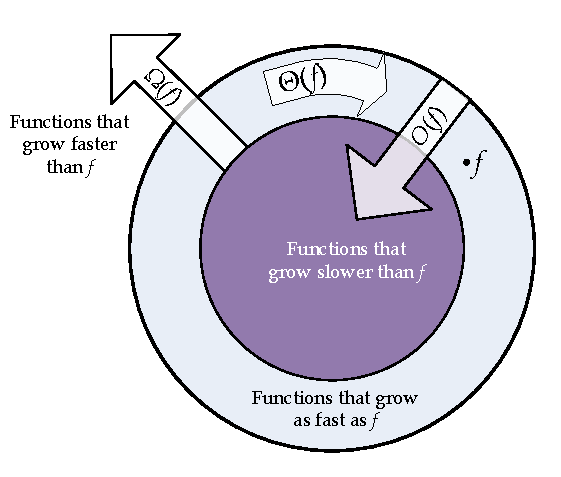
\includegraphics[width=3.2in]{figures/theta.pdf}
\caption{Visualization of the sets $O(f)$, $\Omega(f)$, and $\Theta(f)$.}
\end{center}
\end{figure}

\index{general}{asymptotic operators}
\subsection{Big \emph{O}}\label{sec:bigO}\index{general}{$O$} The first notation we introduce is $O$, pronounced ``big oh''.  The $O$ function takes as input a function, and produces as output the set of all functions that grow no faster than the input function.  The set $O(f)$ is the set of all functions that grow as fast as, or slower than, $f$ grows.  In Figure~\ref{fig-visual}, the $O(f)$ set is represented by everything inside the outer circle.

To define the meaning of $O$ precisely, we need to consider what it means for a function to \emph{grow}.  We want to capture how the output of the function increases as the input to the function increases.  First, we consider a few examples; then we provide a formal definition of $O$.
\begin{descriptionlist}
\item[$f(n) = n + 12$ and $g(n) = n - 7$]\forcenl  
No matter what $n$ value we use, the value of $f(n)$ is greater than the value of $g(n)$.  This doesn't matter for the growth rates, though.  What matters is how the difference between $g(n)$ and $f(n)$ changes as the input values increase.  No matter what values we choose for $n_1$ and $n_2$, we know  $g(n_1) - f(n_1) = g(n_2) - f(n_2) = -19$.  Thus, the growth rates of $f$ and $g$ are identical and  $n - 7$ is in the set $O(n + 12)$, and $n + 12$ is in the set $O(n - 7)$.  
\item[$f(n) = 2n$ and $g(n) = 3n$]\forcenl 
The difference between $g(n)$ and $f(n)$ is $n$.  This difference increases as the input value $n$ increases, but it increases by the same amount as $n$ increases.  So, the growth rate as $n$ increases is $\frac{n}{n} = 1$.  The value of $2n$ is always within a constant multiple of $3n$, so they grow asymptotically at the same rate.  Hence, $2n$ is in the set $O(3n)$ and $3n$ is in the set $O(2n)$.
x\item[$f(n) = n$ and $g(n) = n^2$]\forcenl
The difference between $g(n)$ and $f(n)$ is $n^2 - n = n (n - 1)$.  The growth rate as $n$ increases is $\frac{n (n - 1)}{n} = n - 1$.  The value of $n - 1$ increases as $n$ increases, so $g$ grows faster than $f$.  This means $n^2$ is \emph{not} in $O(n)$ since $n^2$ grows faster than $n$.  The function $n$ is in $O(n^2)$ since $n$ grows slower than $n^2$ grows.
\item[$f(n) = \Fibonacci(n)$ and $g(n) = n$] \forcenl\index{general}{fibonacci}
The $\Fibonacci$ function grows very rapidly.  The value of $\Fibonacci(n+2)$ is more than \emph{double} the value of $\Fibonacci(n)$ since
\begin{displaymath}
\Fibonacci(n+2) = \Fibonacci(n + 1) + \Fibonacci(n)
\end{displaymath}
and $\Fibonacci(n + 1) > \Fibonacci(n)$.  The rate of increase is multiplicative, and must be at least a factor of $\sqrt{2} \approx 1.414$ (since increasing by one twice more than doubles the value).  (In fact, the rate of increase is a factor of $\phi = (1 + \sqrt{5}) / 2 \approx 1.618$, also known as the ``golden ratio''.  This is a rather remarkable result, but explaining why is beyond the scope of this book.)
% TODO: find good reference
This is much faster than the growth rate of $n$, which increases by one when we increase $n$ by one.  So, $n$ is in the set $O(\Fibonacci(n))$, but $\Fibonacci(n)$ is not in the set $O(n)$.
\end{descriptionlist}

\LATER{Make this figure prettier}
\begin{figure}[b]
%\centering
\vspace*{2.0ex} 
\begin{tabular*}{8.0in}{p{2.5in}p{2.5in}p{2in}}
% GNUPLOT: LaTeX picture using EEPIC macros
\setlength{\unitlength}{0.120450pt}
\begin{picture}(1349,1169)(0,0)
\footnotesize
\color{black}
\thicklines \path(389,265)(430,265)
\put(307,265){\makebox(0,0)[r]{$0$}}
\color{black}
\thicklines \path(389,430)(430,430)
\put(307,430){\makebox(0,0)[r]{$20$}}
\color{black}
\thicklines \path(389,594)(430,594)
\put(307,594){\makebox(0,0)[r]{$40$}}
\color{black}
\thicklines \path(389,759)(430,759)
\put(307,759){\makebox(0,0)[r]{$60$}}
\color{black}
\thicklines \path(389,923)(430,923)
\put(307,923){\makebox(0,0)[r]{$80$}}
\color{black}
\thicklines \path(389,1088)(430,1088)
\put(307,1088){\makebox(0,0)[r]{$100$}}
\color{black}
\thicklines \path(484,265)(484,306)
\put(484,182){\makebox(0,0){$2$}}
\color{black}
\thicklines \path(675,265)(675,306)
\put(675,182){\makebox(0,0){$4$}}
\color{black}
\thicklines \path(865,265)(865,306)
\put(865,182){\makebox(0,0){$6$}}
\color{black}
\thicklines \path(1056,265)(1056,306)
\put(1056,182){\makebox(0,0){$8$}}
\color{black}
\thicklines \path(1246,265)(1246,306)
\put(1246,182){\makebox(0,0){$10$}}
\color{black}
\color{black}
\thicklines \path(389,265)(1246,265)
\color{black}
\put(143,676){\makebox(0,0)[l]{\shortstack{�}}}
\color{black}
\color{black}
\put(817,58){\makebox(0,0){$n$}}
\color{black}
\color{black}
\put(1294,517){\makebox(0,0)[l]{$3n$}}
\color{black}
\put(1294,1129){\makebox(0,0)[l]{$n^2$}}
\color{black}
\put(1294,723){\makebox(0,0)[l]{$Fibo(n)$}}
\color{black}
\color{red}
\put(389,290){\circle{12}}
\put(484,314){\circle{12}}
\put(579,339){\circle{12}}
\put(675,364){\circle{12}}
\put(770,388){\circle{12}}
\put(865,413){\circle{12}}
\put(960,438){\circle{12}}
\put(1056,463){\circle{12}}
\put(1151,487){\circle{12}}
\put(1246,512){\circle{12}}
\color{blue}
\put(389,273){\circle*{24}}
\put(484,298){\circle*{24}}
\put(579,339){\circle*{24}}
\put(675,397){\circle*{24}}
\put(770,471){\circle*{24}}
\put(865,561){\circle*{24}}
\put(960,668){\circle*{24}}
\put(1056,792){\circle*{24}}
\put(1151,932){\circle*{24}}
\put(1246,1088){\circle*{24}}
\color{green}
\put(389,273){\makebox(0,0){$\star$}}
\put(484,273){\makebox(0,0){$\star$}}
\put(579,281){\makebox(0,0){$\star$}}
\put(675,290){\makebox(0,0){$\star$}}
\put(770,306){\makebox(0,0){$\star$}}
\put(865,331){\makebox(0,0){$\star$}}
\put(960,372){\makebox(0,0){$\star$}}
\put(1056,438){\makebox(0,0){$\star$}}
\put(1151,545){\makebox(0,0){$\star$}}
\put(1246,718){\makebox(0,0){$\star$}}
\color{black}
\thicklines \path(389,265)(1246,265)
\color{black}
\end{picture}
 &
% GNUPLOT: LaTeX picture using EEPIC macros
\setlength{\unitlength}{0.120450pt}
\begin{picture}(1349,1169)(0,0)
\footnotesize
\color{black}
\thicklines \path(430,265)(471,265)
\put(348,265){\makebox(0,0)[r]{$0$}}
\color{black}
\thicklines \path(430,384)(471,384)
\put(348,384){\makebox(0,0)[r]{$1000$}}
\color{black}
\thicklines \path(430,504)(471,504)
\put(348,504){\makebox(0,0)[r]{$2000$}}
\color{black}
\thicklines \path(430,623)(471,623)
\put(348,623){\makebox(0,0)[r]{$3000$}}
\color{black}
\thicklines \path(430,742)(471,742)
\put(348,742){\makebox(0,0)[r]{$4000$}}
\color{black}
\thicklines \path(430,861)(471,861)
\put(348,861){\makebox(0,0)[r]{$5000$}}
\color{black}
\thicklines \path(430,981)(471,981)
\put(348,981){\makebox(0,0)[r]{$6000$}}
\color{black}
\thicklines \path(559,265)(559,306)
\put(559,182){\makebox(0,0){$4$}}
\color{black}
\thicklines \path(731,265)(731,306)
\put(731,182){\makebox(0,0){$8$}}
\color{black}
\thicklines \path(902,265)(902,306)
\put(902,182){\makebox(0,0){$12$}}
\color{black}
\thicklines \path(1074,265)(1074,306)
\put(1074,182){\makebox(0,0){$16$}}
\color{black}
\thicklines \path(1246,265)(1246,306)
\put(1246,182){\makebox(0,0){$20$}}
\color{black}
\color{black}
\thicklines \path(430,265)(1246,265)
\color{black}
\put(143,676){\makebox(0,0)[l]{\shortstack{�}}}
\color{black}
\color{black}
\put(838,58){\makebox(0,0){$n$}}
\color{black}
\color{black}
\put(1289,325){\makebox(0,0)[l]{$n^2$}}
\color{black}
\put(1289,1072){\makebox(0,0)[l]{$Fibo(n)$}}
\color{black}
\color{red}
\put(430,265){\circle{12}}
\put(473,266){\circle{12}}
\put(516,266){\circle{12}}
\put(559,266){\circle{12}}
\put(602,267){\circle{12}}
\put(645,267){\circle{12}}
\put(688,268){\circle{12}}
\put(731,268){\circle{12}}
\put(774,268){\circle{12}}
\put(817,269){\circle{12}}
\put(859,269){\circle{12}}
\put(902,269){\circle{12}}
\put(945,270){\circle{12}}
\put(988,270){\circle{12}}
\put(1031,270){\circle{12}}
\put(1074,271){\circle{12}}
\put(1117,271){\circle{12}}
\put(1160,271){\circle{12}}
\put(1203,272){\circle{12}}
\put(1246,272){\circle{12}}
\color{blue}
\put(430,265){\circle*{24}}
\put(473,265){\circle*{24}}
\put(516,266){\circle*{24}}
\put(559,267){\circle*{24}}
\put(602,268){\circle*{24}}
\put(645,269){\circle*{24}}
\put(688,271){\circle*{24}}
\put(731,273){\circle*{24}}
\put(774,275){\circle*{24}}
\put(817,277){\circle*{24}}
\put(859,279){\circle*{24}}
\put(902,282){\circle*{24}}
\put(945,285){\circle*{24}}
\put(988,288){\circle*{24}}
\put(1031,292){\circle*{24}}
\put(1074,296){\circle*{24}}
\put(1117,299){\circle*{24}}
\put(1160,304){\circle*{24}}
\put(1203,308){\circle*{24}}
\put(1246,313){\circle*{24}}
\color{green}
\put(430,265){\makebox(0,0){$\star$}}
\put(473,265){\makebox(0,0){$\star$}}
\put(516,265){\makebox(0,0){$\star$}}
\put(559,265){\makebox(0,0){$\star$}}
\put(602,266){\makebox(0,0){$\star$}}
\put(645,266){\makebox(0,0){$\star$}}
\put(688,267){\makebox(0,0){$\star$}}
\put(731,268){\makebox(0,0){$\star$}}
\put(774,269){\makebox(0,0){$\star$}}
\put(817,272){\makebox(0,0){$\star$}}
\put(859,276){\makebox(0,0){$\star$}}
\put(902,282){\makebox(0,0){$\star$}}
\put(945,293){\makebox(0,0){$\star$}}
\put(988,310){\makebox(0,0){$\star$}}
\put(1031,338){\makebox(0,0){$\star$}}
\put(1074,383){\makebox(0,0){$\star$}}
\put(1117,455){\makebox(0,0){$\star$}}
\put(1160,573){\makebox(0,0){$\star$}}
\put(1203,764){\makebox(0,0){$\star$}}
\put(1246,1072){\makebox(0,0){$\star$}}
\color{black}
\thicklines \path(430,265)(1246,265)
\color{black}
\end{picture}
 & \\
\end{tabular*}
\caption{Orders of Growth.}\label{fig:growth}
%\subcapc{Both graphs show the same functions, but scaled for different input ranges.}
\end{figure}

Some of the example functions are plotted in Figure~\ref{fig:growth}.  The $O$ notation reveals the asymptotic behavior of functions.  The functions plotted are the same in both graphs, but the scale of the horizontal axis is different.  In the first graph, the rightmost value of $n^2$ is greatest; for higher input values, the value of $\Fibonacci(n)$ is greatest.  In the second graph, the values of $\Fibonacci(n)$ for input values up to 20 are so large that the other functions appear as nearly flat lines on the graph.

\shortsection{Definition of $O$} The function $g$ is a member of the set $O(f)$ if and only if there exist positive constants $c$ and $n_0$ such that, for all values $n \ge n_0$,
\begin{displaymath}
g(n) \le cf(n).
\end{displaymath}
We can show $g$ is in $O(f)$ using the definition of $O(f)$ by choosing positive constants for the values of $c$ and $n_0$, and showing that the property $g(n) \le cf(n)$ holds for all values $n \ge n_0$.  To show $g$ is not in $O(f)$, we need to explain how, for any choices of $c$ and $n_0$, we can find values of $n$ that are greater than $n_0$ such that $g(n) \le cf(n)$ does not hold.

\begin{examplenobar}{$O$ Examples} We now show the claimed properties are true using the formal definition.  
%\begin{enumerate}[\bfseries a.]
\begin{descriptionlist}
\item[$n-7$ is in $O(n+12)$] \forcenl Choose $c = 1$ and $n_0 = 1$.  Then, we need to show $n-7 \le 1(n+12)$ for all values $n \ge 1$.  This is true, since $n-7 > n+12$ for all values $n$.  
\item[$n+12$ is in $O(n-7)$] \forcenl Choose $c = 2$ and $n_0 = 26$.  Then, we need to show $n+12 \le 2(n-7)$ for all values $n \ge 26$.  The equation simplifies to $n + 12 \le 2n - 14$, which simplifies to $26 \le n$.  This is trivially true for all values $n \ge 26$.
\item[$2n$ is in $O(3n)$]\forcenl Choose $c = 1$ and $n_0 = 1$.  Then, $2n \le 3n$ for all values $n \ge 1$.
\item[$3n$ is in $O(2n)$]\forcenl Choose $c = 2$ and $n_0 = 1$.  Then, $3n \le 2(2n)$ simplifies to $n \le 4/3 n$ which is true for all values $n \ge 1$.
\item[$n$ is in $O(n^2)$]\forcenl Choose $c = 1$ and $n_0 = 1$.  Then $n \le n^2$ for all values $n \ge 1$.
\item[$n^2$ is \bold{not} in $O(n)$]\forcenl We need to show that no matter what values are chosen for $c$ and $n_0$, there are values of $n \ge n_0$ such that the inequality $n^2 \le cn$ does not hold.  For any value of $c$, we can make $n^2 > cn$ by choosing $n>c$.
\item[$n$ is in $O(\Fibonacci(n))$]\forcenl Choose $c = 1$ and $n_0 = 3$.  Then $n \le \Fibonacci(n)$ for all values $n \ge n_0$.
\item[$\Fibonacci(n)$ is \bold{not} in $O(n-2)$]\forcenl No matter what values are chosen for $c$ and $n_0$, there are values of $n \ge n_0$ such that $\Fibonacci(n) > c(n)$.  We know $\Fibonacci(12)=144$, and, from the discussion above, that:
\begin{displaymath}
\Fibonacci(n+2) > 2 * \Fibonacci(n)
\end{displaymath}
This means, for $n>12$, we know $\Fibonacci(n)>n^2$.  So, no matter what value is chosen for $c$, we can choose $n=c$.  Then, we need to show 
\begin{displaymath}
\Fibonacci(n) > n(n)
\end{displaymath}
The right side simplifies to $n^2$.  For $n>12$, we know $\Fibonacci(n) > n^2$.  Hence, we can always choose an $n$ that contradicts the $\Fibonacci(n) \le cn$ inequality by choosing an $n$ that is greater than $n_0$, 12, and $c$.
\end{descriptionlist}
\end{examplenobar}

For all of the examples where $g$ is in $O(f)$, there are many acceptable choices for $c$ and $n_0$.  For the given $c$ values, we can always use a higher $n_0$ value than the selected value.  It only matters that there is some finite, positive constant we can choose for $n_0$, such that the required inequality, $g(n) \le cf(n)$ holds for all values $n \ge n_0$.  Hence, our proofs  work equally well with higher values for $n_0$ than we selected.  Similarly, we could always choose higher $c$ values with the same $n_0$ values.  The key is just to pick any appropriate values for $c$ and $n_0$, and show the inequality holds for all values $n \ge n_0$.

Proving that a function is not in $O(f)$ is usually tougher.  The key to these proofs is that the value of $n$ that invalidates the inequality is selected \emph{after} the values of $c$ and $n_0$ are chosen.  One way to think of this is as a game between two adversaries.  The first player picks $c$ and $n_0$, and the second player picks $n$.  To show the property that $g$ is not in $O(f)$, we need to show that no matter what values the first player picks for $c$ and $n_0$, the second player can always find a value $n$ that is greater than $n_0$ such that $g(n) > cf(n)$.

\begin{exercise}\label{ex:bigo}
For each of the $g$ functions below, answer whether or not $g$ is in the set $O(n)$.  Your answer should include a proof.  If $g$ is in $O(n)$ you should identify values of $c$ and $n_0$ that can be selected to make the necessary inequality hold.  If $g$ is not in $O(n)$ you should argue convincingly that no matter what values are chosen for $c$ and $n_0$ there are values of $n \ge n_0$ such the inequality in the definition of $O$ does not hold.
\begin{subexerciselist}
\item $g(n) = n + 5$
\item $g(n) = .01n$
\item $g(n) = 150n + \sqrt{n}$
\item $g(n) = n^{1.5}$
\item $g(n) = n!$
\end{subexerciselist}
\end{exercise}

\begin{exercise}\goldstar
Given $f$ is some function in $O(h)$, and $g$ is some function not in $O(h)$, which of the following must always be true:
\begin{subexerciselist}
\item For all positive integers $m$, $f(m) \le g(m)$.
\item For some positive integer $m$, $f(m) < g(m)$.
\item For some positive integer $m_0$, and all positive integers $m > m_0$, 
\begin{displaymath}
f(m) < g (m).
\end{displaymath}
\end{subexerciselist}
\end{exercise}

\subsection{Omega}\index{general}{$\Omega$}

The set $\Omega(f)$ (omega) is the set of functions that grow no \emph{slower} than $f$ grows.  So, a function $g$ is in $\Omega(f)$ if $g$ grows as fast as $f$ or faster.   
Constrast this with $O(f)$, the set of all functions that grow no \emph{faster} than $f$ grows. In Figure~\ref{fig-visual}, $\Omega(f)$ is the set of all functions outside the darker circle.

The formal definition of $\Omega(f)$ is nearly identical to the definition of $O(f)$: the only difference is the $\le$ comparison is changed to $\ge$.  

\shortsection{Definition of $\Omega(f)$} The function $g$ is a member of the set $\Omega(f)$ if and only if there exist positive constants $c$ and $n_0$ such that, for all values $n \ge n_0$,
\begin{displaymath}
g(n) \ge cf(n).
\end{displaymath} 

\begin{example}{$\Omega$ Examples}
We repeat selected examples from the previous section with $\Omega$ instead of $O$.  The strategy is similar: we show $g$ is in $\Omega(f)$ using the definition of $\Omega(f)$ by choosing positive constants for the values of $c$ and $n_0$, and showing that the property $g(n) \ge cf(n)$ holds for all values $n \ge n_0$.  To show $g$ is not in $\Omega(f)$, we need to explain how, for any choices of $c$ and $n_0$, we can find a choice for $n \ge n_0$ such that $g(n) < cf(n)$.  

\begin{descriptionlist}
\item[$n-7$ is in $\Omega(n+12)$]\forcenl Choose $c = \frac{1}{2}$ and $n_0 = 26$.  Then, we need to show $n-7 \ge \frac{1}{2} (n+12)$ for all values $n \ge 26$.  This is true, since the inequality simplifies $\frac{n}{2} \ge 13$ which holds for all values $n \ge 26$.  % fixed 2009-12-29, Kristine Dell
%\item $n+12$ is in $\Omega(n-7)$: Choose $c = 1$ and $n_0 = 1$.  

\item[$2n$ is in $\Omega(3n)$]\forcenl Choose $c = \frac{1}{3}$ and $n_0 = 1$.  Then, $2n \ge \frac{1}{3}(3n)$ simplifies to $n \ge 0$ which holds for all values $n \ge 1$.
%\item $3n$ is in $\Omega(2n)$: Choose $c = 1$ and $n_0 = 1$.  Then, $3n \ge 2n$ simplifies to $n \ge 0$ which is true for all values $n \ge 1$.

\item[$n$ is not in $\Omega(n^2)$]\forcenl Whatever values are chosen for $c$ and $n_0$, we can choose $n \ge n_0$ such that $n \ge cn^2$ does not hold.  Choose $n > \frac{1}{c}$ (note that $c$ must be less than 1 for the inequality to hold for any positive $n$, so if $c$ is not less than 1 we can just choose $n \ge 2$).  Then, the right side of the inequality $cn^2$ will be greater than $n$, and the needed inequality $n \ge cn^2$ does not hold.
%\item[$n^2$ is in $\Omega(n)$]\forcenl Choose $c = 1$ and $n_0 = 0$: $n^2 \ge n$ for all $n \ge 0$.
\item[$n$ is not in $\Omega(\Fibonacci(n))$] \forcenl No matter what values are chosen for $c$ and $n_0$, we can choose $n \ge n_0$ such that $n \ge \Fibonacci(n)$ does not hold.  The value of $\Fibonacci(n)$ more than doubles every time $n$ is increased by 2 (see Section~\ref{sec:bigO}), but the value of $c(n)$ only increases by $2c$.  Hence, if we keep increasing $n$, eventually $\Fibonacci(n+1) > c(n-2)$ for any choice of $c$.
%\item $\Fibonacci(n+1)$ is in $\Omega(n-2)$: choose $c = 1$ and $n_0 = 0$: $\Fibonacci(n+1) \ge n-2$ for all $n \ge 0$.
\end{descriptionlist}
\end{example}

%It is instructive to compare the answers here to the ones we got earlier for the same pairs of functions using $O$: for items a, b, c, and d the $g$ function was in %both $O(f)$ and $\Omega(f)$; for items e and g the $g$ function was in $O(f)$ but not in $\Omega(f)$; and for items f and h, the $g$ function was not in $O(f)$ but %was in $\Omega(f)$.  There is no item where the $g$ function is not in either $O(f)$ or $\Omega(f)$: this makes sense since $O(f)$ is the set of functions that %grow no faster than $f$, and $\Omega(f)$ is the set of functions that grow no slower than $f$.  If $g$ grows at the same rate as $f$, it will be in both $O(f)$ and %$\Omega(f)$; if it does not grow at the same rate, it either grows faster than $f$ (it is in $\Omega(f)$), or it grows slower than $f$ (it is in %$O(f)$).\footnote{This is not necessarily the case if the functions are not monotonic; for example, the value of $g(n)$ may oscillate above and below the value of %$f(n)$ such that the inequality properties needed for  $O$ and $\Omega$ are both false for some values $n$ above any $n_0$.  Such functions are not in either $O(f)$ %or $\Omega(f)$, but we are not likely encounter such non-monotonic functions in analyzing programs.} 

\beforeex
\begin{exercise}
Repeat Exercise~\ref{ex:bigo} using $\Omega$ instead of $O$.
\solution{\LATER{}}
\end{exercise}
\afterex

\beforeex
\begin{exercise}
For each part, identify a function $g$ that satisfies the property.
\begin{subexerciselist}
\item $g$ is in $O(n^2)$ but not in $\Omega(n^2)$.
\solution{\LATER{}}
\item $g$ is not in $O(n^2)$ but is in $\Omega(n^2)$.
\solution{\LATER{}}
\item $g$ is in both $O(n^2)$ and $\Omega(n^2)$.
\solution{\LATER{}}
\end{subexerciselist}
\end{exercise}
\afterex


\subsection{Theta}\index{general}{$\Theta$}

The function $\Theta(f)$ denotes the set of functions that grow at the same rate as $f$.  It is the intersection of the sets $O(f)$ and $\Omega(f)$.  Hence, a function $g$ is in $\Theta(f)$ if and only if $g$ is in $O(f)$ and $g$ is in $\Omega(f)$.  In Figure~\ref{fig-visual}, $\Theta(f)$ is the ring between the outer and inner circles.

An alternate definition combines the inequalities for $O$ and $\Omega$:

\shortsection{Definition of $\Theta(f)$} The function $g$ is a member of the set $\Theta(f)$ if any only if there exist positive constants $c_1$, $c_2$, and $n_0$ such that, for all values $n \ge n_0$, 
\begin{displaymath}
c_1 f(n) \ge g(n) \ge c_2 f(n).
\end{displaymath}
If $g(n)$ is in $\Theta(f(n))$, then the sets $\Theta(f(n))$ and $\Theta(g(n))$ are identical.  \cut{We also know $O(f(n)) = O(g(n))$ and $\Omega(f(n)) = \Omega(g(n))$.} If $g(n) \in \Theta(f(n))$ then $g$ and $f$ grow at the same rate, 

\begin{example}{$\Theta$ Examples}
Determining membership in $\Theta(f)$ is simple once we know membership in $O(f)$ and $\Omega(f)$.
\begin{descriptionlist}
\item[$n-7$ is in $\Theta(n+12)$]\forcenl 
Since $n-7$ is in $O(n+12)$ and $n-7$ is in $\Omega(n+12)$ we know $n-7$ is in $\Theta(n+12)$.  Intuitively, $n-7$ increases at the same rate as $n+12$, since adding one to $n$ adds one to both function outputs.  We can also show this using the definition of $\Theta(f)$: choose $c_1 = 1$, $c_2 = \frac{1}{2}$, and $n_0 = 38$. \cut{ We choose the value of $c_1$ as the value of $c$ in the $O(f)$ proof, $c_2$ as the value of $c$ in the $\Omega(f)$ proof, and $n_0$ as the maximum value of the $n_0$ values from the $O(f)$ and $\Omega(f)$ proofs.}
%\item $n+12$ is in $\Theta(n-7)$: $n+12$ is in $O(n-7)$ and in $\Omega(n-7)$.  Choose $c_1 = 2$, $c_2 = 1$, and $n_0 = 1$.
\item[$2n$ is in $\Theta(3n)$]\forcenl $2n$ is in $O(3n)$ and in $\Omega(3n)$.  Choose $c_1 = 1$, $c_2 = \frac{1}{3}$, and $n_0 = 1$.
%\item $3n$ is in $\Theta(2n)$: $3n$ is in $O(2n)$ and in $\Omega(2n)$.  Choose $c_1 = 2$, $c_2 = 1$, and $n_0 = 1$.
\item[$n$ is \bold{not} in $\Theta(n^2)$]\forcenl $n$ is not in $\Omega(n^2)$.  Intuitively, $n$ grows slower than $n^2$ since increasing $n$ by one always increases the value of the first function, $n$, by one, but increases the value of $n^2$ by $2n + 1$, a value that increases as $n$ increases.
\item[$n^2$ is \bold{not} in $\Theta(n)$:] $n^2$ is not in $O(n)$.  
\item[$n-2$ is \bold{not} in $\Theta(\Fibonacci(n+1))$:] $n-2$ is not in $\Omega(n)$.
\item[$\Fibonacci(n)$ is \bold{not} in $\Theta(n)$:] $\Fibonacci(n+1)$ is not in $O(n-2)$.
\end{descriptionlist}
\end{example}

\shortsection{Properties of $O$, $\Omega$, and $\Theta$} Because $O$, $\Omega$, and $\Theta$ are concerned with the asymptotic properties of functions, that is, how they grow as inputs approach infinity, many functions that are different when the actual output values matter generate identical sets with the $O$, $\Omega$, and $\Theta$ functions.  For example, we saw $n-7$ is in $\Theta(n+12)$ and $n+12$ is in $\Theta(n-7)$.  In fact, every function that is in $\Theta(n-7)$ is also in $\Theta(n+12)$.  

More generally, if we could prove $g$ is in $\Theta(an+k)$ where $a$ is a positive constant and $k$ is any constant, then $g$ is also in $\Theta(n)$.  Thus, the set $\Theta(an+k)$ is equivalent to the set $\Theta(n)$.  

We prove $\Theta(an+k) \equiv \Theta(n)$ using the definition of $\Theta$.  To prove the sets are equivalent, we need to show inclusion in both directions.
\begin{descriptionlist}
\item[$\Theta(n) \subseteq \Theta(an+k)$:] For any function $g$, if $g$ is in $\Theta(n)$ then $g$ is in $\Theta(an+k)$. Since $g$ is in $\Theta(n)$ there exist positive constants $c_1$, $c_2$, and $n_0$ such that $c_1 n \ge g(n) \ge c_2 n$.  To show $g$ is also in $\Theta(an+k)$ we find $d_1$, $d_2$, and $m_0$ such that $d_1 (an + k) \ge g(n) \ge d_2 (an+k)$ for all $n \ge m_0$.  Simplifying the inequalities, we need $(ad_1)n + kd_1 \ge g(n) \ge (ad_2)n + kd_2$.  Ignoring the constants for now, we can pick $d_1 = \frac{c_1}{a}$ and $d_2 = \frac{c_2}{a}$.  Since $g$ is in $\Theta(n)$, we know 
\begin{displaymath}
(a\frac{c_1}{a})n \ge g(n) \ge (a\frac{c_2}{a})n
\end{displaymath}
is satisfied.  As for the constants, as $n$ increases they become insignificant.  Adding one to $d_1$ and $d_2$ adds $an$ to the first term and $k$ to the second term. Hence, as $n$ grows, $an$ becomes greater than $k$.  
\item[$\Theta(an + k) \subseteq \Theta(k)$:] For any function $g$, if $g$ is in $\Theta(an+k)$ then $g$ is in $\Theta(n)$. Since $g$ is in $\Theta(an+k)$ there exist positive constants $c_1$, $c_2$, and $n_0$ such that $c_1 (an+k) \ge g(n) \ge c_2 (an+k)$.  Simplifying the inequalities, we have $(ac_1)n + kc_1 \ge g(n) \ge (ac_2)n + kc_2$ or, for some different positive constants $b_1 = ac_1$ and $b_2 = ac_2$ and constants $k_1 = kc_1$ and $k_2=kc_2$, $b_1n + k_1 \ge g(n) \ge b_2 n + k_2$.  To show $g$ is also in $\Theta(n)$, we find $d_1$, $d_2$, and $m_0$ such that $d_1 n \ge g(n) \ge d_2 n$ for all $n \ge m_0$.  If it were not for the constants, we already have this with $d_1 = b_1$ and $d_2 = b_2$.  As before, the constants become inconsequential as $n$ increases.
\end{descriptionlist}
This property also holds for the $O$ and $\Omega$ operators since our proof for $\Theta$ also proved the property for the $O$ and $\Omega$ inequalities.

This result can be generalized to any polynomial.  The set $\Theta(a_0 + a_1 n + a_2 n^2 + ... + a_kn^k)$ is equivalent to $\Theta(n^k)$.  Because we are concerned with the asymptotic growth, only the highest power term of the polynomial matters once $n$ gets big enough.  

\shortex{Repeat Exercise~\ref{ex:bigo} using $\Theta$ instead of $O$.}
\shortex{\label{exercise:thetan} Show that $\Theta(n^2-n)$ is equivalent to $\Theta(n^2)$.}
\shortex{\goldstar Is $\Theta(n^2)$ equivalent to $\Theta(n^{2.1})$?  Either prove they are identical, or prove they are different.}
\shortex{\goldstar Is $\Theta(2^n)$ equivalent to $\Theta(3^n)$?  Either prove they are identical, or prove they are different.}

%% Old chapter 8 starts here.
  
\section{Analyzing Procedures}\label{sec:analyzing}

By considering the asymptotic growth of functions, rather than their actual outputs, the $O$, $\Omega$, and $\Theta$ operators allow us to hide constants and factors that change depending on the speed of our processor, how data is arranged in memory, and the specifics of how our interpreter is implemented.  Instead, we can consider the essential properties of how the running time of the procedures increases with the size of the input.

This section explains how to measure input sizes and running times. To understand the growth rate of a procedure's running time, we need a function that maps the size of the inputs to the procedure to the amount of time it takes to evaluate the application.  First we consider how to measure the input size; then, we consider how to measure the running time.  In Section~\ref{sec:worstcase} we consider \emph{which} input of a given size should be used to reason about the cost of applying a procedure.  Section~\ref{sec:growthrates} provides examples of procedures with different growth rates.  The growth rate of a procedure's running time gives us an understanding of how the running time increases as the size of the input increases. 

\subsection{Input Size}\label{sec:inputsize}\index{general}{measuring input size}

Procedure inputs may be many different types: Numbers, Lists of Numbers, Lists of Lists, Procedures, etc.  Our goal is to characterize the input size with a single number that does not depend on the types of the input.

We use the Turing machine to model a computer, so the way to measure the size of the input is the number of characters needed to write the input on the tape.  The characters can be from any fixed-size alphabet, such as the ten decimal digits, or the letters of the alphabet.  %As we saw in Chapter~\ref{ch:intro}, we can use a sequence of bits to uniquely represent a member of any finite set.  
The number of different symbols in the tape alphabet does not matter for our analysis since we are concerned with orders of growth not absolute values.  Within the $O$, $\Omega$, and $\Theta$ operators, a constant factor does not matter (e.g., $\Theta(n) \equiv \Theta(17n+523)$).  This means is doesn't matter whether we use an alphabet with two symbols or an alphabet with 256 symbols.  With two symbols the input may be 8 times as long as it is with a 256-symbol alphabet, but the constant factor does not matter inside the asymptotic operator.

Thus, we measure the size of the input as the number of symbols required to write the number on a Turing Machine input tape.  To figure out the input size of a given type, we need to think about how many symbols it would require to write down inputs of that type.

\tagpar{Booleans} There are only two Boolean values: \true\ and \false.  Hence, the length of a Boolean input is fixed.

\tagpar{Numbers} Using the decimal number system (that is, 10 tape symbols), we can write a number of magnitude $n$ using $\log_{10} n$ digits.  Using the binary number system (that is, 2 tape symbols), we can write it using $\log_{2} n$ bits.  Within the asymptotic operators, the base of the logarithm does not matter (as long as it is a constant) since it changes the result by a constant factor.  We can see this from the argument above --- changing the number of symbols in the input alphabet changes the input length by a constant factor which has no impact within the asymptotic operators.  \cut{Another way to see this is to use the formula for change logarithm bases:\index{general}{logarithm}
\begin{displaymath}
\log_b x = \frac{1}{\log_a b} \cdot \log_a x
\end{displaymath}
Changing the base of the logarithm multiplies the value by $\frac{1}{\log_a b}$, a constant factor if both logarithm bases are constants.}

\tagpar{Lists} If the input is a List, the size of the input is related to the number of elements in the list.  If each element is a constant size (for example, a list of numbers where each number is between 0 and 100), the size of the input list is some constant multiple of the number of elements in the list.  Hence, the size of an input that is a list of $n$ elements is $cn$ for some constant $c$.  Since $\Theta(cn) = \Theta(n)$, the size of a List input is $\Theta(n)$ where $n$ is the number of elements in the List.  If List elements can vary in size, then we need to account for that in the input size.  For example, suppose the input is a List of Lists, where there are $n$ elements in each inner List, and there are $n$ List elements in the main List.  Then, there are $n^2$ total elements and the input size is in $\Theta(n^2)$.

\subsection{Running Time}

We want a measure of the running time of a procedure that satisfies two properties: (1) it should be robust to ephemeral properties of a particular execution or computer, and (2) it should provide insights into how long it takes evaluate the procedure on a wide range of inputs.  

To estimate the running time of an evaluation, we use the number of steps required to perform the evaluation.  The actual number of steps depends on the details of how much work can be done on each step.  For any particular processor, both the time it takes to perform a step and the amount of work that can be done in one step varies.  When we analyze procedures, however, we usually don't want to deal with these details.  Instead, what we care about is how the running time changes as the input size increases.  This means we can count anything we want as a ``step'' as long as each step is the approximately same size and the time a step requires does not depend on the size of the input.  

The clearest and simplest definition of a step is to use one Turing Machine step.  We have a precise definition of exactly what a Turing Machine can do in one step: it can read the symbol in the current square, write a symbol into that square, transition its internal state number, and move one square to the left or right.  Counting Turing Machine steps is very precise, but difficult because we do not usually start with a Turing Machine description of a procedure and creating one is tedious.  \index{general}{Turing Machine}
\sidequote{Time makes more converts than reason.}{Thomas Paine} \index{people}{Paine, Thomas}

Instead, we usually reason directly from a Scheme procedure (or any precise description of a procedure) using larger steps.  As long as we can claim that whatever we consider a step could be simulated using a constant number of steps on a Turing Machine, our larger steps will produce the same answer within the asymptotic operators.  One possibility is to count the number of times an evaluation rule is used in an evaluation of an application of the procedure.  The amount of work in each evaluation rule may vary slightly (for example, the evaluation rule for an if expression seems more complex than the rule for a primitive) but does not depend on the input size.  

Hence, it is reasonable to assume all the evaluation rules to take constant time.  This does not include any additional evaluation rules that are needed to apply one rule.  For example, the evaluation rule for application expressions includes evaluating every subexpression.  Evaluating an application constitutes one work unit for the application rule itself, plus all the work required to evaluate the subexpressions.  In cases where the bigger steps are unclear, we can always return to our precise definition of a step as one step of a Turing Machine.  

\subsection{Worst Case Input}\label{sec:worstcase}

A procedure may have different running times for inputs of the same size.  

For example, consider this procedure that takes a List as input and outputs the first positive number in the list:
\begin{schemedisplay}
(define (list-first-pos p)
  (if (null? p) (error "No positive element found")
      (if (> (car p) 0) (car p) (list-first-pos (cdr p)))))
\end{schemedisplay}

If the first element in the input list is positive, evaluating the application of \scheme|list-first-pos| requires very little work.  It is not necessary to consider any other elements in the list if the first element is positive.  On the other hand, if none of the elements are positive, the procedure needs to test each element in the list until it reaches the end of the list (where the base case reports an error).  

In our analyses we usually consider the \definition{worst case} input.  For a given size, the worst case input is the input for which evaluating the procedure takes the most work.  By focusing on the worst case input, we know the maximum running time for the procedure.  Without knowing something about the possible inputs to the procedure, it is safest to be pessimistic about the input and not assume any properties that are not known (such as that the first number in the list is positive for the \scheme|first-pos| example).

In some cases, we also consider the \emph{average case} input.  Since most procedures can take infinitely many inputs, this requires understanding the distribution of possible inputs to determine an ``average'' input.  This is often necessary when we are analyzing the running time of a procedure that uses another helper procedure.  If we use the worst-case running time for the helper procedure, we will grossly overestimate the running time of the main procedure.  Instead, since we know how the main procedure uses the helper procedure, we can more precisely estimate the actual running time by considering the actual inputs.  We see an example of this in the analysis of how the \scheme|+| procedure is used by \scheme|list-length| in Section~\ref{sec:linear}.

\section{Growth Rates}\label{sec:growthrates}\index{general}{growth rates}

Since our goal is to understand how the running time of an application of a procedure is related to the size of the input, we want to devise a function that takes as input a number that represents the size of the input and outputs the maximum number of steps required to complete the evaluation on an input of that size.  Symbolically, we can think of this function as:
\begin{quote}
$\MaxSteps$: \var{Number} $\rightarrow$ \var{Number}
\end{quote}
where \textsl{Proc} is the name of the procedure we are analyzing.  Because the output represents the \emph{maximum} number of steps required, we need to consider the worst-case input of the given size.

Because of all the issues with counting steps exactly, and the uncertainty about how much work can be done in one step on a particular machine, we cannot usually determine the exact function for $\MaxSteps$.  Instead, we characterize the running time of a procedure with a set of functions denoted by an asymptotic operator.  Inside the $O$, $\Omega$, and $\Theta$ operators, the actual time needed for each step does not matter since the constant factors are hidden by the operator; what matters is how the number of steps required grows as the size of the input grows.  

Hence, we will characterize the running time of a procedure using a set of functions produced by one of the asymptotic operators.  The $\Theta$ operator provides the most information.  Since $\Theta(f)$ is the intersection of $O(f)$ (no faster than) and $\Omega(f)$ (no slower than), knowing that the running time of a procedure is in $\Theta(f)$ for some function $f$ provides much more information than just knowing it is in $O(f)$ or just knowing that it is in $\Omega(f)$.  Hence, our goal is to characterize the running time of a procedure using the set of functions defined by $\Theta(f)$ of some function $f$.  
%For a given procedure, we should nearly always be able to get a tight ($\Theta$) bound on its running time.  %In Chapter~\ref{ch:intractability}, we consider the harder problem of determining the running time the best possible procedure that solves a particular problem.

The rest of this section provides examples of procedures with different growth rates, from slowest (no growth) through increasingly rapid growth rates.  The growth classes described are important classes that are commonly encountered when analyzing procedures, but these are only examples of growth classes.  Between each pair of classes described here, there are an unlimited number of different growth classes.

\subsection{No Growth: Constant Time}\label{sec:no-growth}\label{sec:constant-time}

If the running time of a procedure does not increase when the size of the input increases, the procedure must be able to produce its output by looking at only a constant number of symbols in the input.  Procedures whose running time does not increase with the size of the input are known as \definition{constant time} procedures.  Their running time is in $O(1)$ --- it does not grow at all.  By convention, we use $O(1)$ instead of $\Theta(1)$ to describe constant time.  Since there is no way to grow slower than not growing at all, $O(1)$ and $\Theta(1)$ are equivalent.

We cannot do much in constant time, since we cannot even examine the whole input.  A constant time procedure must be able to produce its output by examining only a fixed-size part of the input.  Recall that the input size measures the number of squares needed to represent the input.  No matter how long the input is, a constant time procedure can look at no more than some fixed number of squares on the tape, so cannot even read the whole input.

%\shortsection{List procedures} 
An example of a constant time procedure is the built-in procedure \scheme|car|.  When \scheme|car| is applied to a non-empty list, it evaluates to the first element of that list.  No matter how long the input list is, all the \scheme|car| procedure needs to do is extract the first component of the list.  So, the running time of \scheme|car| is in $O(1)$.\footnote{Since we are speculating based on what \scheme|car| does, not examining how \scheme|car| a particular Scheme interpreter actually implements it, we cannot say definitively that its running time is in $O(1)$.  It would be rather shocking, however, for an implementation to implement \scheme|car| in a way such that its running time that is not in $O(1)$. The implementation of \scheme|scar| in Section~\ref{sec:makingpairs} is constant time: regardless of the input size, evaluating an application of it involves evaluating a single application expression, and then evaluating an if expression.}  Other built-in procedures that involve lists and pairs that have running times in $O(1)$ include \scheme|cons|, \scheme|cdr|, \scheme|null?|, and \scheme|pair?|.  None of these procedures need to examine more than the first pair of the list.

%Most procedures that take numbers as inputs are not constant time since most operations on numbers depend on the whole number.  For example, there is no way to correctly add two numbers without %completely reading all the digits in both numbers.  

%\shortsection{Boolean procedures} All sensible procedures that have only Booleans as inputs are constant time.  This is because the size of a Boolean input is a constant.  Since there is no way to grow %the size of a Boolean input, the running time of a procedure that takes only Boolean inputs should not grow either.  For example, the \scheme|logical-and| procedure from Chapter~\ref{ch:machines} takes %two Boolean inputs.  Evaluating it involves evaluating one if expression, so the running time is constant.

%\shortsection{Number procedures} 

%There are some operations we can do on numbers in constant time, however.  
%
%For example, the \scheme|zero?| procedure takes a number as its input and outputs a Boolean indicating whether or not the input number is zero.  Whether it is possible to implement \scheme|zero?| in %constant time depends on how numbers are represented.  If numbers are represented with no leading zeros (that is, \scheme|0043| is not a valid number), then all \scheme|zero?| needs to do is look at the %first digit, so it can be done in constant time.  We will more examples in the next section involving arithmetic operations where one of the numbers is a constant.

\subsection{Linear Growth}\label{sec:linear}

When the running time of a procedure increases by a constant amount when the size of the input grows by one, the running time of the procedure grows \definition{linearly} with the input size.  If the input size is $n$, the running time is in $\Theta(n)$.  If a procedure has running time in $\Theta(n)$, doubling the size of the input will approximately double the execution time.

An example of a procedure that has linear growth is the elementary school addition algorithm from Section~\ref{sec:binaryarithmetic}.  To add two $d$-digit numbers, we need to perform a constant amount of work for each digit.  The number of steps required grows linearly with the size of the numbers (recall from Section~\ref{sec:inputsize} that the \emph{size} of a number is the number of input symbols needed to represent the number\cut{, which is logarithmic in the magnitude of the number}).

Many procedures that take a List as input have linear time growth.  A procedure that does something that takes constant time with every element in the input List, has running time that grows linearly with the size of the input since adding one element to the list increases the number of steps by a constant amount.  Next, we analyze three list procedures, all of which have running times that scale linearly with the size of their input.

\begin{examplenobar}{Append}\label{example:time-list-append} Consider the \scheme|list-append| procedure (from Example~\ref{example:append}):
\begin{schemedisplay}
(define (list-append p q)
  (if (null? p) q (cons (car p) (list-append (cdr p) q))))
\end{schemedisplay}

Since \scheme|list-append| takes two inputs, we need to be careful about how we refer to the input size.  We use $n_p$ to represent the number of elements in the first input, and $n_q$ to represent the number of elements in the second input.  So, our goal is to define a function $\RunningTimeL(n_p, n_q)$ that captures how the maximum number of steps required to evaluate an application of \scheme|list-append| scales with the size of its input.

To analyze the running time of \scheme|list-append|, we examine its body which is an if expression.  The predicate expression applies the \scheme|null?| procedure with is constant time since the effort required to determine if a list is \scheme|null| does not depend on the length of the list.  When the predicate expression evaluates to \schemeresult|true|, the alternate expression is just \scheme|q|, which can also be evaluated in constant time.  

Next, we consider the alternate expression.  It includes a recursive application of \scheme|list-append|.  Hence, the running time of the alternate expression is the time required to evaluate the recursive application plus the time required to evaluate everything else in the expression.  The other expressions to evaluate are applications of \scheme|cons|, \scheme|car|, and \scheme|cdr|, all of which is are constant time procedures.  

So, we can defined the total running time recursively as:
\begin{displaymath}
\RunningTimeL(n_p, n_q) = C + \RunningTimeL(n_p - 1, n_q)
\end{displaymath}
where \var{C} is some constant that reflects the time for all the operations besides the recursive call.  Note that the value of $n_q$ does not matter, so we simplify this to:
\begin{displaymath}
\RunningTimeL(n_p) = C + \RunningTimeL(n_p - 1).
\end{displaymath}
This does not yet provide a useful characterization of the running time of \scheme|list-append| though, since it is a circular definition.  To make it a recursive definition, we need a base case.  The base case for the running time definition is the same as the base case for the procedure: when the input is \scheme|null|.  For the base case, the running time is constant:
\begin{displaymath}
\RunningTimeL(0) = C_0
\end{displaymath}
where $C_0$ is some constant.

To better characterize the running time of \scheme|list-append|, we want a closed form solution.  For a given input $n$, $\RunningTime(n)$ is $C + C + C + C + \ldots + C + C_0$ where there are $n-1$ of the $C$ terms in the sum.  This simplifies to $(n-1)C + C_0 = nC - C + C_0 = nC + C_2$.  We do not know what the values of $C$ and $C_2$ are, but within the asymptotic notations the constant values do not matter.  The important property is that the running time scales linearly with the value of its input.  Thus, the running time of \scheme|list-append| is in $\Theta(n_p)$ where $n_p$ is the number of elements in the first input.

Usually, we do not need to reason at quite this low a level.  Instead, to analyze the running time of a recursive procedure it is enough to determine the amount of work involved in each recursive call (excluding the recursive application itself) and multiply this by the number of recursive calls.  For this example, there are $n_p$ recursive calls since each call reduces the length of the \scheme|p| input by one until the base case is reached.  Each call involves only constant-time procedures (other than the recursive application), so the amount of work involved in each call is constant.  Hence, the running time is in $\Theta(n_p)$.  Equivalently, the running time for the \scheme|list-append| procedure scales linearly with the length of the first input list. 

\end{examplenobar}

\begin{examplenobar}{Length}\label{example:time-list-length} Consider the \scheme|list-length| procedure from Example~\ref{example:length}:

\begin{schemedisplay}
(define (list-length p) (if (null? p) 0 (+ 1 (list-length (cdr p)))))
\end{schemedisplay}

This procedure makes one recursive application of \scheme|list-length| for each element in the input \scheme|p|.  If the input has $n$ elements, there will be $n+1$ total applications of \scheme|list-length| to evaluate (one for each element, and one for the \scheme|null|).  So, the total work is in $\Theta(n \cdot \textrm{work for each recursive application})$.

To determine the running time, we need to determine how much work is involved in each application.  Evaluating an application of \scheme|list-length| involves evaluating its body, which is an if expression.  To evaluate the if expression, the predicate expression, \scheme|(null? p)|, must be evaluated first.  This requires constant time since the \scheme|null?| procedure has constant running time (see Section~\ref{sec:no-growth}).   The consequent expression is the primitive expression, \scheme|0|, which can be evaluated in constant time.    The alternate expression, \scheme|(+ 1 (list-length (cdr p)))|, includes the recursive call.  There are $n+1$ total applications of \scheme|list-length| to evaluate, the total running time is $n+1$ times the work required for each application (other than the recursive application itself).

The remaining work is evaluating \scheme|(cdr p)| and evaluating the \scheme|+| application.  The \scheme|cdr| procedure is constant time. 
Analyzing the running time of the \scheme|+| procedure application is more complicated.  

\shortsection{Cost of Addition} Since \scheme|+| is a built-in procedure, we need to think about how it might be implemented.  Following the elementary school addition algorithm (from Section~\ref{sec:binaryarithmetic}), we know we can add any two numbers by walking down the digits.  The work required for each digit is constant; we just need to compute the corresponding result and carry bits using a simple formula or lookup table.  The number of digits to add is the maximum number of digits in the two input numbers.    Thus, if there are $b$ digits to add, the total work is in $\Theta(b)$.  In the worst case, we need to look at all the digits in both numbers.  In general, we cannot do asymptotically better than this, since adding two arbitrary numbers might require looking at all the digits in both numbers.  

But, in the \scheme|list-length| procedure the \scheme|+| is used in a very limited way: one of the inputs is always \schemeresult|1|.  We might be able to add \scheme|1| to a number without looking at all the digits in the number.  Recall the addition algorithm: we start at the rightmost (least significant) digit, add that digit, and continue with the carry.  If one of the input numbers is \scheme|1|, then once the carry is zero we know now of the more significant digits will need to change.  In the worst case, adding one requires changing every digit in the other input.  For example, \scheme|(+ 99999 1)| is \scheme|100000|.  In the best case (when the last digit is below \scheme|9|), adding one requires only examining and changing one digit.  
\sidepicturenocap{0.5}{images/odometer-iStock_000006968970XSmall.jpg}\label{picture:odometer}%{Worst Case}{}

Figuring out the average case is more difficult, but necessary to get a good estimate of the running time of \scheme|list-length|.  We assume the numbers are represented in binary, so instead of decimal digits we are counting bits (this is both simpler, and closer to how numbers are actually represented in the computer).  Approximately half the time, the least significant bit is a \bit{0}, so we only need to examine one bit.  When the last bit is not a \bit{0}, we need to examine the second least significant bit (the second bit from the right): if it is a \bit{0} we are done; if it is a \bit{1}, we need to continue.  

We always need to examine one bit, the least significant bit.  Half the time we also need to examine the second least significant bit.  Of those times, half the time we need to continue and examine the next least significant bit.  This continues through the whole number.  Thus, the expected number of bits we need to examine is,
\begin{displaymath}
1 + \frac{1}{2}\left(1 + \frac{1}{2} \left(1 + \frac{1}{2}\left(1 + \frac{1}{2}\left(1 + \ldots\right)\right)\right)\right)
\end{displaymath}
where the number of terms is the number of bits in the input number, $b$.  Simplifying the equation, we get:
\begin{displaymath}
1 + \frac{1}{2} + \frac{1}{4} + \frac{1}{8} + \frac{1}{16} + \ldots + \frac{1}{2^b}
\end{displaymath}
No matter how large $b$ gets, this value is always less than $2$.  So, on average, the number of bits to examine to add \scheme|1| is constant: it does not depend on the length of the input number.   %Although adding two arbitrary values cannot be done in constant time, adding \scheme|1| to an arbitrary value can, on average, be done in constant time.

This result generalizes to addition where one of the inputs is any constant value.  Add\-ing any constant $C$ to a number $n$ is equivalent to adding one $C$ times.  Since adding one is a constant time procedure, adding one $C$ times can also be done in constant time for any constant $C$.  \cut{Another way to see this is to note that the constant $C$ can be written in $\log_2 C$ bits.  Hence, we always need to look at the rightmost $\log_2 C$ bits of the input number, but only need to look beyond those bits when there are carries.  The frequency of carries after the next most significant bit is the same as if we are adding \scheme|1|.  So, on average, we only need to look at a constant number of bits to add a constant to any number.}

Excluding the recursive application, the \scheme|list-length| application involves applications of two constant time procedures: \scheme|cdr| and adding one using \scheme|+|.  Hence, the total time needed to evaluate one application of \scheme|list-length|, excluding the recursive application, is constant.  %It does not depend on the length of the input list.  

There are $n+1$ total applications of \scheme|list-length| to evaluate total, so the total running time is $c(n+1)$ where $c$ is the amount of time needed for each application.  The set $\Theta(c(n+1))$ is identical to the set $\Theta(n)$, so the running time for the length procedure is in $\Theta(n)$ where $n$ is the length of the input list. 
\end{examplenobar}
%%\clearpage %%!

\begin{examplenobar}{Accessing List Elements}\label{example:time-list-get-element}  Consider the \scheme|list-get-element| procedure from Example~\ref{example:list-get-element}\LATER{REF}:
\begin{schemedisplay}
(define (list-get-element p n) 
   (if (= n 1)
       (car p)
       (list-get-element (cdr p) (- n 1))))
\end{schemedisplay}
The procedure takes two inputs, a List and a Number selecting the element of the list to get.  Since there are two inputs, we need to think carefully about the input size.  We can use variables to represent the size of each input, for example $s_p$ and $s_n$ for the size of $p$ and $n$ respectively.  In this case, however, only the size of the first input really matters.  

The procedure body is an if expression.  The predicate uses the built-in \scheme|=| procedure to compare $n$ to \scheme|1|.  The worst case running time of the \scheme|=| procedure is linear in the size of the input: it potentially needs to look at all bits in the input numbers to determine if they are equal.  Similarly to \scheme|+|, however, if one of the inputs is a constant, the comparison can be done in constant time.  To compare a number of any size to \scheme|1|, it is enough to look at a few bits.  If the least significant bit of the input number is not a \bit{1}, we know the result is \scheme|false|.  If it is a \bit{1}, we need to examine a few other bits of the input number to determine if its value is different from \scheme|1| (the exact number of bits depends on the details of how numbers are represented).  So, the \scheme|=| comparison can be done in constant time.

If the predicate is \schemeresult|true|, the base case applies the \scheme|car| procedure, which has constant running time.  The alternate expression involves the recursive calls, as well as evaluating \scheme|(cdr p)|, which requires constant time, and \scheme|(- n 1)|.  The \scheme|-| procedure is similar to \scheme|+|: for arbitrary inputs, its worst case running time is linear in the input size, but when one of the inputs is a constant the running time is constant.  This follows from a similar argument to the one we used for the \scheme|+| procedure (Exercise~\ref{exercise:subtraction} asks for a more detailed analysis of the running time of subtraction).  So, the work required for each recursive call is constant.

The number of recursive calls is determined by the value of $n$ and the number of elements in the list $p$.  In the best case, when $n$ is \scheme|1|, there are no recursive calls and the running time is constant since the procedure only needs to examine the first element.  Each recursive call reduces the value passed in as $n$ by \scheme|1|, so the number of recursive calls scales linearly with $n$ (the actual number is $n - 1$ since the base case is when $n$ equals \scheme|1|).  But, there is a limit on the value of $n$ for which this is true.  If the value passed in as $n$ exceeds the number of elements in $p$, the procedure will produce an error when it attempts to evaluate \scheme|(cdr p)| for the empty list.  This happens after $s_p$ recursive calls, where $s_p$ is the number of elements in $p$.  Hence, the running time of \scheme|list-get-element| does not grow with the length of the input passed as $n$; after the value of $n$ exceeds the number of elements in $p$ it does not matter how much bigger it gets, the running time does not continue to increase.  

Thus, the worst case running time of \scheme|list-get-element| grows linearly with the length of the input list.  Equivalently, the running time of \scheme|list-get-element| is in $\Theta(s_p)$ where $s_p$ is the number of elements in the input list.
\end{examplenobar}

\beforeex
\begin{exercise}
Explain why the \scheme|list-map| procedure from Section~\ref{sec:examining-lists} has running time that is linear in the size of its List input.  Assume the procedure input has constant running time.
\solution{\LATER{}}
\end{exercise}
\afterex

\beforeex
\begin{exercise}
Consider the \scheme|list-sum| procedure (from Example~5.2)\LATER{\ref{example:list-sum})}:
\begin{schemedisplay}
(define (list-sum p) (if (null? p) 0 (+ (car p) (list-sum (cdr p)))))
\end{schemedisplay}
What assumptions are needed about the elements in the list for the running time to be linear in the number if elements in the input list?
\solution{\LATER{}}
\end{exercise}
\afterex

\sidepicturenocap{0.30}{images/AVM-Printomatic-0-9-9-reading-mockup.jpg}%{Voting Machine Counter}{}%http://dvice.com/archives/2008/10/the_last_thing.php
\beforesplitex
\begin{exercise}
For the decimal six-digit odometer (shown in the picture on page~\pageref{picture:odometer}), we measure the amount of work to add one as the total number of wheel digit turns required.  For example, going from \bits{000000} to \bits{000001} requires one work unit, but going from \bits{000099} to \bits{000100} requires three work units.
\begin{subexerciselist}
\item What are the worst case inputs?
\solution{\LATER{}}
\item What are the best case inputs?
\solution{\LATER{}}
\item \goldstar On average, how many work units are required for each mile?  Assume over the lifetime of the odometer, the car travels 1,000,000 miles.
\solution{\LATER{}}
\item Lever voting machines were used by the majority of American voters in the 1960s, although they are not widely used today.  Most level machines used a three-digit odometer to tally votes.  Explain why candidates ended up with 99 votes on a machine far more often than 98 or 100 on these machines.
\solution{\LATER{}}
\end{subexerciselist}
\end{exercise}
\aftersplitex

\beforesplitex
\begin{exercise}\label{exercise:subtraction}\goldstar 
The \scheme|list-get-element| argued by comparison to \scheme|+|, that the \scheme|-| procedure has constant running time when one of the inputs is a constant.  Develop a more convincing argument why this is true by analyzing the worst case and average case inputs for \scheme|-|.
\solution{\LATER{}}
\end{exercise}
\aftersplitex

\beforesplitex
\begin{exercise}\goldstar Our analysis of the work required to add one to a number argued that it could be done in constant time.  Test experimentally if the DrRacket \scheme|+| procedure actually satisfies this property.  Note that one \scheme|+| application is too quick to measure well using the \scheme|time| procedure, so you will need to design a procedure that applies \scheme|+| many times without doing much other work.
\solution{\LATER{}}
\end{exercise}
\aftersplitex

\LATER{excursion on grey codes}

\subsection{Quadratic Growth}

If the running time of a procedure scales as the square of the size of the input, the procedure's running time grows \definition{quadratically}.  
Doubling the size of the input approximately quadruples the running time.  The running time is in $\Theta(n^2)$ where $n$ is the size of the input.  

A procedure that takes a list as input has running time that grows quadratically if it goes through all elements in the list once for every element in the list.  For example, we can compare every element in a list of length $n$ with every other element using $n(n-1)$ comparisons.  This simplifies to $n^2 - n$, but $\Theta(n^2 - n)$ is equivalent to $\Theta(n^2)$ since as $n$ increases only the highest power term matters (see Exercise~\ref{exercise:thetan}).  

%%!\clearpage %%!
\begin{examplenobar}{Reverse}\label{example:list-reverse-time}
Consider the \scheme|list-reverse| procedure defined in Section~\ref{sec:generic}:
\begin{schemedisplay}
(define (list-reverse p)
  (if (null? p) null (list-append (list-reverse (cdr p)) (list (car p)))))
\end{schemedisplay}

To determine the running time of \scheme|list-reverse|, we need to know how many recursive calls there are and how much work is involved in each recursive call.  Each recursive application passes in \scheme|(cdr p)| as the input, so reduces the length of the input list by one.  Hence,  applying \scheme|list-reverse| to a input list with $n$ elements involves $n$ recursive calls.  

The work for each recursive application, excluding the recursive call itself, is applying \scheme|list-append|.  The first input to \scheme|list-append| is the output of the recursive call.  As we argued in Example~\ref{example:time-list-append}, the running time of \scheme|list-append| is in $\Theta(n_p)$ where $n_p$ is the number of elements in its first input.  So, to determine the running time we need to know the length of the first input list to \scheme|list-append|.  For the first call, \scheme|(cdr p)| is the parameter, with length $n-1$; for the second call, there will be $n-2$ elements; and so forth, until the final call where \scheme|(cdr p)| has $0$ elements.  The total number of elements in all of these calls is: 
\begin{displaymath}
(n-1) + (n-2) + \ldots + 1 + 0.  
\end{displaymath}
The average number of elements in each call is approximately $\frac{n}{2}$.  Within the asymptotic operators the constant factor of $\frac{1}{2}$ does not matter, so the average running time for each recursive application is in $\Theta(n)$.  

There are $n$ recursive applications, so the total running time of \scheme|list-reverse| is $n$ times the average running time of each recursive application: \[n \cdot \Theta(n) = \Theta(n^2).\]  Thus, the running time is quadratic in the size of the input list.
\end{examplenobar}

\begin{examplenobar}{Multiplication} Consider the problem of multiplying two numbers.  The elementary school long multiplication algorithm works by multiplying each digit in $b$ by each digit in $a$, aligning the intermediate results in the right places, and summing the results:

\groupcontent{
\begin{tabbing} 
\qquad \= \qquad \qquad    \= \qquad\qquad \= \qquad\qquad \= \qquad\qquad \= \qquad\qquad \= \qquad\qquad \= \qquad\qquad \= \qquad\qquad \= \qquad\qquad \= \qquad\qquad \= \qquad\qquad \=   \kill
     
          \>         \>         \>      \>          \> $a_{n-1}$  \> $\cdots$  \> $a_1$  \> $a_0$ \\
          \>         \>         \>     \>    \qquad $\times$     \> $b_{n-1}$  \> $\cdots$  \> $b_1$  \> $b_0$ \\[-0.5ex]
          \>         \>          \>     \>  \> \rule{5.4cm}{0.2mm} \\[0ex]
           \>        \>          \>     \>          \> $a_{n-1}b_0$   \> $\cdots$ \> $a_1b_0$ \> $a_0b_0$ \\
            \>       \>          \>    \> $a_{n-1}b_1$   \> $\cdots$ \> $a_1b_1$ \> $a_0b_1$ \>         \\
      \> \qquad $+$   \> $a_{n-1}b_{n-1}$  
                        \> \quad $\cdots$ 
                                  \> $a_1b_{n-1}$ 
                                           \> $a_0b_{n-1}$   \>                \>          \>          \>            \> \\
     \> \rule{11.5cm}{0.2mm} \\[0ex]
    \> $r_{2n-1}$       \> $r_{2n-2}$ \>  \quad $\cdots$                \>     $\cdots$          \>    $r_3$      \>   $r_2$ \>  $r_1$ \> $r_0$ \\
\end{tabbing}
}

If both input numbers have $n$ digits, there are $n^2$ digit multiplications, each of which can be done in constant time.  \sidepicturenocap{0.5}{images/multiplication-iStock_000003661783Small.jpg}
The intermediate results will be $n$ rows, each containing $n$ digits.  So, the total number of digits to add is $n^2$: 1 digit in the ones place, 2 digits in the tens place, $\ldots$, $n$ digits in the $10^{n-1}$s place, $\ldots$, 2 digits in the $10^{2n-3}$s place, and 1 digit in the $10^{2n-2}$s place.  Each digit addition requires constant work, so the total work for all the digit additions is in $\Theta(n^2)$.  Adding the work for both the digit multiplications and the digit additions, the total running time for the elementary school multiplication algorithm is quadratic in the number of input digits, $\Theta(n^2)$ where $n$ is the number if digits in the inputs.

This is not the fastest known algorithm for multiplying two numbers, although it was the best algorithm known until 1960.  In 1960, Anatolii Karatsuba discovers a multiplication algorithm with running time in $\Theta(n^{\log_2 3})$.  Since $\log_2 3 < 1.585$ this is an improvement over the $\Theta(n^2)$ elementary school algorithm.  In 2007, Martin F\"{u}rer discovered an even faster algorithm for multiplication.\footnote{Martin F\"{u}rer, Faster Integer Multiplication, \emph{ACM Symposium on Theory of Computing}, 2007.}  It is not yet known if this is the fastest possible multiplication algorithm, or if faster ones exist. 
 
\end{examplenobar}

\beforeex
\begin{exercise}
\goldstar Analyze the running time of the elementary school long division algorithm.
\solution{\LATER{}}
\end{exercise}
\afterex

%\sidepicturenocap{0.3}{images/frustration-iStock_000003621931Small.jpg}
%\ex{\doublegoldstar
%Is it possible to define a \scheme|list-reverse| procedure that behaves identically to the procedure above, but has running time in $\Theta(n)$ where $n$ is the number of elements in the input list?  Either define such a procedure, or explain why it cannot be done.
%}
\beforeex
\begin{exercise}
\goldstar
Define a Scheme procedure that multiplies two multi-digit numbers (without using the built-in \scheme|*| procedure except to multiply single-digit numbers).  Strive for your procedure to have running time in $\Theta(n)$ where $n$ is the total number of digits in the input numbers.
\solution{\LATER{}}
\end{exercise}
\afterex

\beforeex
\begin{exercise}
\quadgoldstar
Devise an asymptotically faster general multiplication algorithm than F\"{u}rer's, or prove that no faster algorithm exists.
\solution{\LATER{}}
\end{exercise}
\afterex

 % fixed 2009-12-29

\cut{
\subsection{Polynomial Growth}\label{sec:polynomialgrowth}
A \emph{polynomial} function is a function that is the sum of powers of one or more variables multiplied by coefficients.  For example, 
\begin{displaymath}
a_k n^k + ... + a_3 n^3 + a_2 n^2 + a_1 n + a_0
\end{displaymath}
is a polynomial where the variable is $n$ and the coefficients are $a_0, a_1, ..., a_k$.  Within the $O$, $\Omega$ and $\Theta$ operators, only the term with the largest exponent matters.  For high enough $n$, all the other terms become insignificant.  An easy way to see this is to observe that $n^k$ is $n \cdot n^{k-1}$ for all positive integers $k$.  So, whatever the $a_{k-1}$ coefficient is, once $n > a_{k-1}$ the value of $n^k > a_{k-1}n^{k-1}$.  So, the polynomial above is in $\Theta(n^k)$ which is equivalent to $\Theta(a_kn^k + ... + a_3 n^3 + a_2 n^2 + a_1 n + a_0)$ for all positive constants $a_0, \ldots, a_k$.  

All of the slower growth rates in this section are polynomials: constant growth is a polynomial where the highest exponent is 0, linear growth is a polynomial where the highest exponent is 1, and quadratic grow is a polynomial where the highest exponent is 2.  We can have procedures where the running time grows as a higher polynomial.  The next example analyzes a procedure whose running time grows cubically with the size of its input. 
% It is not the fastest procedure for solving the given problem, however. Later, we show a procedure that defines the same function but has quadratic running time.

%\TODO{Better Example}

\begin{example}{Satisfying pair}\label{example:list-satisfying-pair}
The \scheme{list-satisfying-pair} procedure, defined below, takes as inputs a test procedure and a list.  The test procedure is a procedure that takes two inputs and produces a Boolean value.  If there are any pairs of elements in the list for which the test procedure evaluates to true, the output is a  pair of two elements in the list for which the test procedure evaluates to true.  Otherwise, the output is \schemeresult|false| to indicate there is no satisfying pair.

Here are some example evaluations:
\begin{code}
\scheme|> (list-satisfying-pair = (list 1 3 2 4 6 1))|\\
\schemeresult|(1 . 1)|\\
\scheme|> (list-satisfying-pair = (list 1 3 2 4 6 7))|\\
\schemeresult|false|\\
\scheme|> (list-satisfying-pair (lambda (a b) (= a (* b 2)))|\\
\scheme|                        (list 2 3 5 7 11 13))|\\
\schemeresult|false|\\
\scheme|> (list-satisfying-pair (lambda (a b) (= a (* b b)))|\\
\scheme|                        (list 3 4 5 6 7 8 9 10 11))|\\
\schemeresult|(9 . 3)|
\end{code}

We can define \scheme|list-satisfying-pair| by using \scheme|list-get-element| to select elements in turn to try all possible pairs.  

\begin{schemedisplay}
(define (list-satisfying-pair cf p)
  (define (list-satisfying-pair-iter i j)
    (if (> i (list-length p))
        false
        (if (> j (list-length p))
            (list-satisfying-pair-iter (+ i 1) 1)
            (if (and (not (= i j)) 
                     (cf (list-get-element p i) (list-get-element p j)))
                (cons (list-get-element p i) (list-get-element p j))
                (list-satisfying-pair-iter i (+ j 1))))))
  (list-satisfying-pair-iter 1 1))      
\end{schemedisplay}

The inner definition defines the \scheme|list-satisfying-pair-iter| procedure that takes two inputs, \scheme|i| and \scheme|j|, Numbers used to represent the indices of elements in the list to compare.  It also uses the two parameters to the outer \scheme|list-satisfying-pair| procedure: \scheme|cf|, the Procedure used to test if a pair of inputs satisfy some property, and \scheme|p|, the input List.

To check all possible pairs, we need to evaluate the test procedure for every pair of values \scheme|i| and \scheme|j| that correspond to elements in the input list.  We use $n$ to represent the number of elements in the input list.  Since there are $n$ possible values for \scheme|i| and $n$ possible values for \scheme|j|, this amounts to $n^2$ total comparisons.  The number of recursive calls to \scheme|list-satisfying-pair-iter| should match this.  The recursive definition is a bit complex since there are two different recursive calls.  The first base case is when \scheme|i| exceeds the length of the input list.  When this is true, it means all possible pairs have been tried without finding a satisfying pair, so the output is \schemeresult|false|.  The second base case is when \scheme|j|, the second index, exceeds the length of the list.  This happens when the procedure has finished trying the comparison procedure with all pairs for a given first element (the value of \scheme|i|).  To continue, the recursive call, \scheme|(list-satisfying-pair-iter (+ i 1) 1)| passes in the next value for \scheme|i| and resets the value for the \scheme|j| parameter to \schemeresult|1|.  This happens $n$ times.  

The other recursive call is done when \scheme|(> j (list-length p))| evaluates to \schemeresult|false|: \scheme|(list-satisfying-pair-iter i (+ j 1))|.  The value passed in as \scheme|i| does not change, but the value passed as \scheme|j| increases by \scheme|1|.  Since \scheme|j| starts at \scheme|1|, the number of recursive calls required before the predicate is false is $n$.  After these $n$ calls, the recursive call that increases \scheme|i| by \scheme|1| and resets \scheme|j| to \scheme|1| is used.  Hence, the total number of recursive calls is $n^2$.

So, to determine the running time of \scheme|list-satisfying-pair| we need to estimate the running time of each application of \scheme|list-satisfying-pair-iter| (excluding the recursive call) and multiply that by $n^2$.  The worst (and most common) path through \scheme|list-satisfying-pair-iter| is the path where the first two predicate expressions are false, and the third one is true.  Along this path, we need to evaluate \scheme|(> i (list-length p))|, \scheme|(> j (list-length p))|, \scheme|(and (not (= i j)) (cf (list-get-element p i) (list-get-element p j)))|, and \scheme|(cons (list-get-element p i) (list-get-element p j))|.  We consider the running time of each expression in turn; the total running time for each \scheme|list-satisfying-pair-iter| application is the sum of the running times of each expression.

The first two expressions use the \scheme|>| procedure to compare the index value to the length of the list.  The running time of \scheme|list-length| is linear in the number of elements in the input list, so this involves $\Theta(n)$ work.  The less than comparison can be done by examining the bits of the input numbers from most-significant to least-significant bit.  In the worst case, all bits in the input numbers need to be examined.  This occurs when all the bits are the same, or all the bits except the last bit are the same.  The value of the first input is some number between $1$ and $n+1$; the value of the second input is always $n$.  Hence, the size of the input to \scheme|<| is $\Theta(\log n)$ and the running time for evaluating each \scheme|>| expression is in $\Theta(\log n)$.  The total running time for evaluating \scheme|(> i (list-length p))| is $\Theta(n + \log n)$ which is equivalent to $\Theta(n)$ since as $n$ increases, the $\log n$ term becomes much smaller than $n$ (that is, $1.1n > (n + \log n)$ for $n > 100$).  The running time for the second comparison expression is also in $\Theta(n)$.  

The third expression involves applications of the Boolean procedure \scheme|not|, which is constant time since it takes Boolean inputs; the comparison procedure, \scheme|cf|, which we assume is constant time; and two applications of \scheme|list-get-element|, which we analyzed in Example~\ref{example:time-list-get-element} to have running time that is linear in the number of elements in the input List in the worst case.  The running time for \scheme|list-get-element| scales linearly with the value of the second input, up to the length of the first input.  On average, the values of \scheme|i| and \scheme|j| will be the average length of the list = $n/2$, so the expected running time of each	 call is also in $\Theta(n)$.  This means the total running time for \scheme|list-satisfying-pair| is in $\Theta(n^3)$ since there are $\Theta(n^2)$ recursive calls, and each one has running time in $\Theta(n)$.  So, the running time for this expression is in $O(1) + O(1) + \Theta(n) + \Theta(n) = \Theta(n)$.

The fourth expression, \scheme|(cons (list-get-element p i) (list-get-element p j))|, also involves two applications of \scheme|list-get-element| and the constant time procedures \scheme|cons|.  Hence, its running time is in $\Theta(n)$.

The total running time to evaluate all four expressions is the sum of their running times: $\Theta(n) + \Theta(n) + \Theta(n) + \Theta(n)$, which is equivalent to $\Theta(n)$.  Since there are $n^2$ recursive calls, the total running time for \scheme|list-satisfying-pair| is in $n^2 \cdot \Theta(n) = \Theta(n^3)$.
\end{example}


\begin{exercise} \doublegoldstar
The provided definition of \scheme|list-satisfying-pair| has cubic running time, but it is possible to implement a procedure with the same behavior that has running time in $\Theta(n^2)$ where $n$ is the number of elements in the input list.  Write a definition of \scheme|list-satisfying-pair| that has quadratic running time, and explain why the running time of your procedure is quadratic.
\end{exercise}
}

\subsection{Exponential Growth}\index{general}{exponential}

If the running time of a procedure scales as a power of the size of the input, the procedure's running time grows \emph{exponentially}.  When the size of the input increases by one, the running time is multiplied by some constant factor.  The growth rate of a function whose output is multiplied by $w$ when the input size, $n$, increases by one is $w^n$.  Exponential growth is very fast---it is not feasible to evaluate applications of an exponential time procedure on large inputs.  

%A common instance of exponential growth is when the running time is in $\Theta(2^n)$.  This occurs when the running time doubles when the input size increases by one.  

For a surprisingly large number of interesting problems, the best known algorithm has exponential running time.  Examples of problems like this include finding the best route between two locations on a map (the problem mentioned at the beginning of Chapter~\ref{ch:problems}), the pegboard puzzle (Exploration~\ref{exploration:pegboard}, solving generalized versions of most other games such as Suduko and Mine\-sweeper, and finding the factors of a number.  Whether or not it is possible to design faster algorithms that solve these problems is the most important open problem in computer science.\cut{, which we will return to in \chintrac.}\index{general}{intractability}

%Next, we provide two examples of procedures that have exponential running time.

\begin{examplenobar}{Factoring} A simple way to find a factor of a given input number is to exhaustively try all possible numbers below the input number to find the first one that divides the number evenly.  
The \scheme|find-factor| procedure takes one number as input and outputs the lowest factor of that number (other than \scheme|1|):
\begin{schemedisplay}
(define (find-factor n)
  (define (find-factor-helper v)
    (if (= (modulo n v) 0) v (find-factor-helper (+ 1 v))))
  (find-factor-helper 2))
\end{schemedisplay}

The \scheme|find-factor-helper| procedure takes two inputs, the number to factor and the current guess.  Since all numbers are divisible by themselves, the \scheme|modulo| test will eventually be \true\ for any positive input number, so the maximum number of recursive calls is \scheme|n|, the magnitude of the input to \scheme|find-factor|.  The magnitude of \scheme|n| is exponential in its size, so the number of recursive calls is in $\Theta(2^b)$ where $b$ is the number of bits in the input.  This means even if the amount of work required for each recursive call were constant, the running time of the \scheme|find-factor| procedure is still exponential in the size of its input.  

The actual work for each recursive call is not constant, though, since it involves an application of \scheme|modulo|.  The \scheme|modulo| built-in procedure takes two inputs and outputs the remainder when the first input is divided by the second input.  Hence, it output is \scheme|0| if \scheme|n| is divisible by \scheme|v|.  Computing a remainder, in the worst case, at least involves examining every bit in the input number, so scales at least linearly in the size of its input\footnote{In fact, it computing the remainder requires performing division, which is quadratic in the size of the input.}.  This means the running time of \scheme|find-factor| is in $\Omega(2^b)$: it grows at least as fast as $2^b$.

There are lots of ways we could produce a faster procedure for finding factors: stopping once the square root of the input number is reached since we know there is no need to check the rest of the numbers, skipping even numbers after \scheme|2| since if a number is divisible by any even number it is also divisible by \scheme|2|, or using advanced sieve methods.  This techniques can improve the running time by constant factors, but there is no known factoring algorithm that runs in faster than exponential time.  The security of the widely used RSA encryption algorithm depends on factoring being hard.  If someone finds a fast factoring algorithm it would put the codes used to secure Internet commerce at risk.\footnote{The movie \emph{Sneakers} is a fictional account of what would happen if someone finds a faster than exponential time factoring algorithm.}
\end{examplenobar}

\begin{example}{Power Set}  The \definition{power set} of a set $S$ is the set of all subsets of $S$.  For example, the power set of $\{1, 2, 3\}$ is 
$\{\{\}, \{1\}, \{2\}, \{3\}, \{1, 2\}, \{1, 3\}, \{2, 3\}, \{1, 2, 3\}\}$.

The number of elements in the power set of $S$ is $2^{|S|}$ (where $|S|$ is the number of elements in the set $S$).  

Here is a procedure that takes a list as input, and produces as output the power set of the elements of the list:

\begin{schemedisplay}
(define (list-powerset s)
  (if (null? s) (list null)
      (list-append (list-map (lambda (t) (cons (car s) t)) 
                             (list-powerset (cdr s)))
                   (list-powerset (cdr s)))))
\end{schemedisplay}

The \scheme|list-powerset| procedure produces a List of Lists.  Hence, for the base case, instead of just producing \scheme|null|, it produces a list containing a single element, \scheme|null|.  In the recursive case, we can produce the power set by appending the list of all the subsets that include the first element, with the list of all the subsets that do not include the first element.  For example, the powerset of $\{1, 2, 3\}$ is found by finding the powerset of $\{2, 3\}$, which is \{\{\}, \{2\}, \{3\}, \{2, 3\}\}, and taking the union of that set with the set of all elements in that set unioned with $\{1\}$.  

An application of \scheme|list-powerset| involves applying \scheme|list-append|, and two recursive applications of \scheme|(list-powerset (cdr s))|.  Increasing the size of the input list by one, \emph{doubles} the total number of applications of \scheme|list-powerset| since we need to evaluate \scheme|(list-powerset (cdr s))| twice.  The number of applications of \scheme|list-powerset| is $2^n$ where $n$ is the length of the input list.\footnote{Observant readers will note that it is not really necessary to perform this evaluation twice since we could do it once and reuse the result.  Even with this change, though, the running time would still be in $\Theta(2^n)$.}

The body of \scheme|list-powerset| is an if expression.  The predicate applies the constant-time procedure, \scheme|null?|.  The consequent expression, \scheme|(list null)| is also constant time.  The alternate expression is an application of \scheme|list-append|.  From Example~\ref{example:time-list-append}, we know the running time of \scheme|list-append| is $\Theta(n_p)$ where $n_p$ is the number of elements in its first input.  The first input is the result of applying \scheme|list-map| to a procedure and the List produced by \scheme|(list-powerset (cdr s))|.  The length of the list output by \scheme|list-map| is the same as the length of its input, so we need to determine the length of \scheme|(list-powerset (cdr s))|.  

We use $n_s$ to represent the number of elements in \scheme|s|.  The length of the input list to \scheme|map| is the number of elements in the power set of a size $n_s-1$ set: $2^{n_s-1}$.  But, for each application, the value of $n_s$ is different.  Since we are trying to determine the total running time, we can do this by thinking about the total length of all the input lists to \scheme|list-map| over all of the \scheme|list-powerset|.  In the input is a list of length $n$, the total list length is
$2^{n-1} + 2^{n - 2} + ... + 2^1 + 2^0$, which is equal to $2^{n}-1$.  So, the running time for all the \scheme|list-map| applications is in $\Theta(2^n)$.  

The analysis of the \scheme|list-append| applications is similar.  The length of the first input to \scheme|list-append| is the length of the result of the \scheme|list-powerset| application, so the total length of all the inputs to append is $2^n$.  

Other than the applications of \scheme|list-map| and \scheme|list-append|, the rest of each \scheme|list-powerset| application requires constant time.  So, the running time required for $2^n$ applications is in $\Theta(2^n)$.  The total running time for \scheme|list-powerset| is the sum of the running times for the \scheme|list-powerset| applications, in $\Theta(2^n)$; the \scheme|list-map| applications, in $\Theta(2^n)$; and the \scheme|list-append| applications, in $\Theta(2^n)$.  Hence, the total running time is in $\Theta(2^n)$.

In this case, we know there can be no faster than exponential procedure that solves the same problem, since the size of the output is exponential in the size of the input.  Since the most work a Turing Machine can do in one step is write one square, the size of the output provides a lower bound on the running time of the Turing Machine.  The size of the powerset is $2^n$ where $n$ is the size of the input set.  Hence, the fastest possible procedure for this problem has at least exponential running time.  
\end{example}


\LATER{
\begin{example}{Primes}\label{example:primes}
A prime number is a number greater than 1 that has no positive integer divisors other than 1 and itself.  To determine if $n$ is a prime number, we can try dividing $n$ by every number between 2 and $n-1$.  If we find a number that divides $n$ with no remainder, then $n$ is composite (that is, not prime).  If there are no numbers other than 1 and $n$ that divide $n$ with no remainder, then $n$ is prime.  Examples of prime numbers include 2, 3, 5, 61, 7177, and $2^{43112609}-1$ (a 12,978,189-digit number found in August 2008 that is the largest known prime number as of February 2009).  

The \scheme|is-prime?| procedure takes a positive integer as its input and outputs true if and only if the input number is prime:
\begin{schemedisplay}
(define (is-prime? n)
  (define (is-prime-iter? n try)
    (if (= n try)
        true
        (if (zero? (modulo n try))
            false
            (is-prime-iter? n (+ try 1)))))
  (is-prime-iter? n 2))
\end{schemedisplay}

In the worst case, \scheme|n| is prime, and all numbers must be attempted before the base case is reached.  The number of recursive applications of \scheme|is-prime-iter?| is \scheme|(- n 2)| (since we start with \scheme|try| as 2).  Each application involves applying \scheme|=|, \scheme|zero?|, \scheme|modulo|, and \scheme|+| (with a constant value).  The applications of \scheme|zero?| and \scheme|+| (with a constant) are constant time, but the applications of \scheme|=| and \scheme|modulo| scale with the input size.  In the worst case, the \scheme|=| procedure needs to compare all the bits in the input numbers.  The number of bits in \scheme|n| is $\log_2 v_n$ where $v_n$ is the value of \scheme|n|.  The value of \scheme|try| is between 2 and \scheme|n|.  So, the maximum number of bits to compare in the \scheme|=| procedure is $2 \log_2 v_n$.  Hence, its running time is in $\Theta(\log v_n)$.  The \scheme|modulo| procedure takes two Numbers as inputs, and outputs the remainder resulting from dividing the first input number by the second input number.    We could implement \scheme|modulo| by performing long division and keeping just the remainder as the final result.  The number of steps required to perform long division scales with the number of digits in the divisor.  For each step, we need to perform a multiplication of a single digit times the dividend.  If we perform long multiplication, the number of steps scales with the number of digits.  So, the running time of a straightforward implementation of \scheme|modulo| would be in $\Theta(\log v_n \log v_m)$ where $v_n$ is the value of the first input, and $v_m$ is the value of the second input.  In the worst case, the average value of \scheme|try| is $\frac{v_n}{2}$, so the running time for the straightfoward \scheme|modulo| procedure is in $\Theta((\log v_n)^2)$.  

As explained in Section~\ref{sec:inputsize}, however, we want to know how the running time scales as the \emph{size} of the input increases.  If the input is a list of constant-sized elements, the size of the input scales with the number of elements in the list.  When the input is a number, the size of the input scales with the number if digits in the input.  If our numbers are written in base 10, increasing the input size by one increases the value of the input by a factor of 10.  The size of the input is $\log v$ where $v$ is the value of the input.  The value of the input, $v$, can be up to $10^d - 1$ where $d$ is the number of digits in the input.  So, if \scheme|is-prime?| is in $\Theta(n)$ where $n$ is the value of the input, it is in $\Theta(10^d)$ where $d$ is the size (number of digits) of the input.  Hence, the \scheme|is-prime?| procedure has running time that grows exponentially in the size of the input.

We could improve our \scheme|is-prime?| implementation by stopping once we reach a value greater than the square root of the input.  This would reduce the number of recursive applications to $\Theta(\sqrt{n})$ where $n$ is the value of the input.  The growth rate is still exponential, however.  The square root of $\Theta(10^d)$ is $\Theta((\sqrt{10})^d) ~= \Theta(\sqrt{3.16}^d)$.
\end{example}

\LATER{
\begin{example}{Exponentiation}\label{example:exponentiation}
Consider the problem of computing $a^b$ for two positive integers, $a$ and $b$.  A simple procedure does this by multiplying $a$ by itself $b$ times:
\begin{schemedisplay}
(define (power a b)
  (if (= b 0)
      1
      (* a (power a (- b 1)))))
\end{schemedisplay}
To analyze the running time of \scheme|power|, we multiply the number of recursive calls by the amount of work involved in each call (excluding the recursive call itself).  We use $v_a$ and $v_b$ to represent the values of $a$ and $b$ respectively.  Since $a$ and $b$ are Numbers, their values are up to $2^n$ where $n$ is the number of bits in each number.

Each recursive call reduces the value passed as the \scheme|b| input by \scheme|1| until the base case where \scheme|b| is \schemeresult|0| is reached, so there are $v_b$ recursive calls.  Each call involves two other applications: the \scheme|-| procedure applied to \scheme|b| and \scheme|1|, and the \scheme|*| procedure applied to \scheme|a| and the result of the recursive call.  As we argued in Example~\ref{example:list-get-element-time}, the subtraction procedure has constant running time when one of its parameters is a constant.  In Example~\ref{example:multiplication}, we saw that there is a multiplication procedure with running time in $\Theta(n^2)$ where $n$ is the number of digits in its inputs.  If that procedure is used to implement the built-in \scheme|*| procedure, the running time for each recursive call is in $\Theta$

  
For the multiplication procedure, we consider the elementary school multiplication algorithm.  To multiply two 

The subtraction has constant time.  

\end{example}
}
\LATER{add some reasonable exercises}

\begin{exercise} \triplegoldstar
Devise a procedure for testing primality whose running time grows slower than exponentially.\footnote{Until 2002 it was generally believed that a primality test with running time faster than exponential did not exist.  Then, Manindra Agrawal and two undergraduate students working on their senior thesis projects, Neeraj Kayal and Nitin Saxena, developed such an algorithm and proved that it was correct.  See Folkmar Bornemann, \emph{PRIMES Is in P: A Breakthrough for ``Everyman''}, Notices of the AMS, Volume 50, Number 5, May 2003; and Manindra Agrawal, Neeraj Kayal and Nitin Saxena, \emph{Primes is in P}, Annals of Mathematics, Volume 160, Number 2, September 2004.}
\end{exercise}

\begin{exercise} \quadgoldstar
Devise a procedure for factoring an input value whose running time grows slower than exponentially.\footnote{No such procedure is currently known, but no one has proven it can't be done either\cut{ or even that it is as hard as solving the pegboard puzzle, although some computer scientists believe that it is (see \chintrac)}.  The security of the most widely used public-key cryptosystems, including those that form the basis of nearly every secure Internet transaction, depends on no such procedure existing.}
\end{exercise}
}

\subsection{Faster than Exponential Growth}

We have already seen an example of a procedure that grows faster than exponentially in the size of the input: the \scheme|fibo| procedure at the beginning of this chapter!  Evaluating an application of \scheme|fibo| involves $\Theta(\phi^n)$ recursive applications where $n$ is the magnitude of the input parameter.  The size of a numeric input is the number of bits needed to express it, so the value $n$ can be as high as $2^b - 1$ where $b$ is the number of bits.  Hence, the running time of the \scheme|fibo| procedure is in $\Theta(\phi^{2^b})$ where $b$ is the size of the input.  This is why we are still waiting for \scheme|(fibo 60)| to finish evaluating. 	

\subsection{Non-terminating Procedures}\label{sec:nonterminating}

All of the procedures so far in the section are algorithms: they may be slow, but they are guaranteed to eventually finish if one can wait long enough.  Some procedures never terminate.  For example,
\begin{schemedisplay}
(define (run-forever) (run-forever))
\end{schemedisplay}
defines a procedure that never finishes.  Its body calls itself, never making any progress toward a base case.  The running time of this procedure is effectively infinite since it never finishes.  

\section{Summary}                              

Because the speed of computers varies and the exact time required for a particular application depends on many details, the most important property to understand is how the work required scales with the size of the input.   The asymptotic operators provide a convenient way of understanding the cost involved in evaluating a procedure applications.  

Procedures that can produce an output only touching a fixed amount have constant running times.  Procedures whose running times increase by a fixed amount when the input size increases by one have linear (in $\Theta(n)$) running times.  Procedures whose running time quadruples when the input size doubles have quadratic (in $\Theta(n^2)$) running times.  Procedures whose running time doubles when the input size increases by one have exponential (in $\Theta(2^n)$) running times.  Procedures with exponential running time can only be evaluated for small inputs.

Asymptotic analysis, however, must be interpreted cautiously.  For large enough inputs, a procedure with running time in $\Theta(n)$ is always faster than a procedure with running time in $\Theta(n^2)$.  But, for an input of a particular size, the $\Theta(n^2)$ procedure may be faster.  Without knowing the constants that are hidden by the asymptotic operators, there is no way to accurately predict the actual running time on a given input.

\cut{So far, we have analyzed the running times of a known procedures.  A deeper question concerns the running time of the best possible procedure that solves a particular problem.  We explore that question in \chintrac.}

\beforeex
\begin{exercise}
Analyze the asymptotic running time of the \scheme|list-sum| procedure (from Example~\ref{example:list-sum}):
\begin{schemedisplay}
(define (list-sum p)
   (if (null? p) 
       0 
       (+ (car p) (list-sum (cdr p)))))
\end{schemedisplay}
You may assume all of the elements in the list have values below some constant (but explain why this assumption is useful in your analysis).
\solution{\LATER{}}
\end{exercise}
\afterex

\beforeex
\begin{exercise}
Analyze the asymptotic running time of the \scheme|factorial| procedure (from Example~\ref{ex:factorial}):
\begin{schemedisplay}
(define (factorial n) (if (= n 0) 1 (* n (factorial (- n 1)))))
\end{schemedisplay}
Be careful to describe the running time in terms of the \emph{size} (not the magnitude) of the input.
\solution{\LATER{}}
\end{exercise}
\afterex

\beforeex
\begin{exercise}
Consider the \scheme|intsto| problem (from Example~\ref{example:intsto}).
\begin{subexerciselist}
\item \goldstar Analyze the asymptotic running time of this \scheme|intsto| procedure:
\begin{schemedisplay}
(define (revintsto n)
  (if (= n 0) 
      null 
      (cons n (revintsto (- n 1)))))
(define (intsto n) (list-reverse (revintsto n)))
\end{schemedisplay}
\item \goldstar Analyze the asymptotic running time of this \scheme|instto| procedure:
\begin{schemedisplay}
(define (intsto n) 
   (if (= n 0) null (list-append (intsto (- n 1)) (list n))))
\end{schemedisplay}
\item Which version is better?
\item \doublegoldstar Is there an asymptotically faster \scheme|intsto| procedure?
\end{subexerciselist}
\solution{\LATER{}}
\end{exercise}
\afterex

\beforeex
\begin{exercise}
Analyze the running time of the \scheme|board-replace-peg| procedure (from Exploration~\ref{exploration:pegboard}):\index{general}{pegboard puzzle}
\begin{schemedisplay}
(define (row-replace-peg pegs col val)
  (if (= col 1) (cons val (cdr pegs))
      (cons (car pegs) (row-replace-peg (cdr pegs) (- col 1) val))))
(define (board-replace-peg board row col val)
  (if (= row 1) (cons (row-replace-peg (car board) col val) (cdr board))
      (cons (car board) (board-replace-peg (cdr board) (- row 1) col val))))
\end{schemedisplay}
\solution{\LATER{}}
\end{exercise}
\afterex

\beforeex
\begin{exercise}
Analyze the running time of the \scheme|deep-list-flatten| procedure from Section~\ref{sec:listsoflists}:
\begin{schemedisplay}
(define (deep-list-flatten p)
  (if (null? p) null
      (list-append (if (list? (car p))
                       (deep-list-flatten (car p))
                       (list (car p)))
                   (deep-list-flatten (cdr p)))))
\end{schemedisplay}
\solution{\LATER{}}
\end{exercise}
\afterex

\beforeex
\begin{exercise}\goldstar 
Find and correct at least one error in the \emph{Orders of Growth} section of the Wikipedia page on \emph{Analysis of Algorithms} (\url{http://en.wikipedia.org/wiki/Analysis_of_algorithms}).  This is rated as \goldstar now (July 2011), since the current entry contains many fairly obvious errors.  Hopefully it will soon become a \triplegoldstar challenge, and perhaps, eventually will become impossible!
\solution{\LATER{}}
\end{exercise}
\afterex


\LATER{size of input - TM tape - better examples - pegboard puzzle}

\end{schemeregion}

%% this chapter now continues in ch8-time.tex